\documentclass[]{report}
\usepackage{amsmath}
\usepackage{amsfonts}
\usepackage{amssymb}
\usepackage{textcomp}
\usepackage{graphicx}
\usepackage{float}
\usepackage{hyperref}
\usepackage[a4paper, margin = 1in]{geometry}

\usepackage[draft]{todonotes}


%Commands used in text, edit here and the document will populate with correct value.
\newcommand{\projectName}{CEPAD }
\newcommand{\payLoadMass}{2.5Kgs }

%*******************************TITLE PAGE*******************************%

\title{Development of a Close Quarter Collision Protected Aerial Drone}
\author{Angus Steele} 

%*******************************START OF DOCUMENT*******************************%

\begin{document}

\maketitle

%*******************************BEGIN THE ABSTRACT*******************************%

\chapter*{Abstract}
\todo[inline]{Incomplete}
The need for robots is evident. High costs of maintenance. High costs of shut-downs for personnel Inspections

%*******************************DOCUMENT LISTS*******************************%

\tableofcontents
%\listoffigures giving issues
\listoftables

%*******************************SELF GENERATED GLOSSARY*******************************%

\chapter*{Glossary}
\begin{enumerate}
%\item Close-Quarter Explosion Protected Aerial Drone (CEPAD)
\item Micro Aerial Vehicles (MAV)
\item Unmanned Aerial System (UAS)
\item Unmanned Aerial Vehicle (UAV)
%\item IECEx (International Electrotechnical Commission for Explosive Atmospheres)
%\item ATEX (Atmosph\`{e}res Explosives)
\item Disk Loading (DL)
\item Power Loading (PL)
%\item South African Bureau of Standards (SABS)
%\item South African National Standards (SANS)
%\item International Organisation of Standards (ISO)
\item Degree of Freedom (DOF)

\item On Board Computer (OBC)
\item Ground Control Station (GCS)
\end{enumerate}

%*******************************CONSISTENCY RULES*******************************%
\newpage

\todo[inline]{RULES FOR CONSISTENCY:}
\todo[inline]{}
\todo[inline]{Figure always with a capital F}
\todo[inline]{Equation, use eqref (or put in brackets) and don't say equation unless it's the beginning of a sentence}
\todo[inline]{Image citation done inline as well as "Taken from (X) in caption"}
\todo[inline]{Equation citation done inline only}
\todo[inline]{Section always with a capital S}

\todo[inline]{}
%*******************************INCLUDE DIFFERENT CHAPTERS*******************************%


\chapter{Literature Study}
In this chapter research is conducted to determine the viability and 


\section{History}
\subsection{Micro Aerial Vehicles}
Flight has long been a phenomenon man has attempted to harness and understand. There are numerous methods of obtaining flight and these all come with their own advantages and disadvantages. As technologies advance they have a tendency to scale down in size, cost and complexity. In the realm of aerial vehicles this has resulted in the development of various micro aerial vehicles, or MAVs \cite{Leishman}. Having significantly lower Reynold's numbers than traditional big aircraft meant that the flow characteristics of these designs would differ. These small craft represent both a technology challenge and a potential new vehicle class that may have substantial societal impact" \cite{NewMAV}

In the realm of MAVs the rotor winged craft brings certain advantages to the table. For environments were high levels of manoeuvrability are required, or even a situation where the platform might need to remain still a rotary design should be considered \cite{Bohorquez}


Specifying that the robot must work in a close quarter environment limits the choice of drive systems \cite{CQAR}. 
For example a fixed wing aircraft would not be a feasible design due to the lack of manoeuvrability and inability to hover. The limited control behind a ducted fan design limits the usefulness in more delicate missions. Due to space requirements in the design specifications, lighter than air vehicles (such as blimps) have not been considered.

This leaves a rotor wing design which is discussed in detail below. The modern day rotor wing aircraft plays a unique role in new age aviation \cite{Leishman} and is required in an application where the platform might need to stand still \cite{Bohorquez}. 

\todo[inline]{When more theory is applicable must add to this section}


%RESEARCH INTO ROTOR THEORY

\section{Flight Theory}
Flight is a broad term and can be seen from as simple a concept as hot smoke rising to a bird flapping its wings. The reality is that flight even encompasses a rugby ball, kicked by Joel Stransky, flying through the air to win South Africa the Rugby World Cup. Although all different forms of flight, the examples above will have a very similar force diagram as seen in figure \ref{IM_FlightForces}.

\begin{figure}
\centering
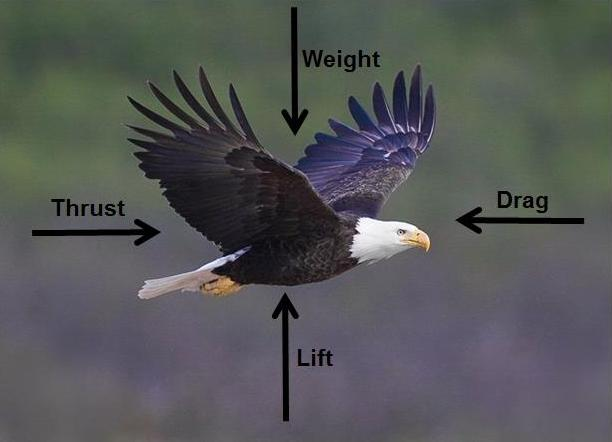
\includegraphics[height = 6cm]{Images/Literature/Bird}
\caption{Force diagram of basic components of flight (Picture adapted from National Geographic Website)}
\label{IM_FlightForces}
\end{figure}

From the force diagram it can be intuitively seen that to increase the velocity of a body in air, the lift must exceed the weight. Kevin Sablan gives a good summary of the forces in \cite{TheoryofFlight}.
Weight is directly determined by the object's mass and the relevant gravity coefficient, $W = mg$. Lift counteracts this weight in an attempt to boost the body into the air. Upward acceleration is only achieved once lift exceeds weight, if they are equal the body will be in a state of hover. From the lift equation seen in equation \ref{EQ_Lift} only a body with velocity can obtain lift. In a rotorcraft, like a helicopter, the rotating blades move through the air and generate lift, the amount generated is governed by equation \ref{EQ_Lift}. 

As seen in figure \ref{IM_Helicopter} the main rotor system, which consists of these rotating blades, is directly coupled to the fuselage and the entire vehicle is lifted into the air. In a fixed wing aircraft if the vehicle is stationery, according to the equation, lift must be zero as there are no moving components. 

\begin{equation}
\label{EQ_Lift}
Lift = C_L(\frac{1}{2} \rho V^2) S
\end{equation}

To propel the body forward the thrust must exceed the value of the drag force acting directly against its velocity vector. Thrust is calculated by combining multiple fields of physics, the effect of thrust can be best summarised by Newton's second law of motion, $F=ma$. The force is generated through interaction with the surrounding atmosphere. Newton's third law agrees that by accelerating large masses of air, thrust is generated in the opposite direction. In the case of a gliding bird, the thrust will equal to zero and the bird will gradually slow down until it flaps its wings again to produce more thrust. This loss of speed is due to drag. Similar to lift, drag varies with velocity as shown in equation (\ref{EQ_Drag}).

\begin{equation}
\label{EQ_Drag}
Drag = C_D (\frac{1}{2} \rho V^2) A
\end{equation}

The coefficient of drag ($C_D$) is determined by the way the object interacts with the air flow, this will comprise of smoothness values as well as shape. 


\subsection{Fundamental Principles of Flow}
Flow is created by any body moving through a medium be it air, water or sand. Therefore any object with an airborne trajectory will be in part governed by the laws of flow. To better understand the principles behind flight, certain theories of flow must be understood.

\subsubsection{Continuity Equation and Bernoulli's Principle}
The continuity equation is used in varying fields of study, it dictates the behaviour of certain phenomenon, or better said their ability to not change. Daniel Bernoulli observed that the mass flow of a flowing medium will follow the laws of continuity in the form of equation \eqref{EQ_Bernoulli}. To do this he observed the conservation of mass flow in a closed system, as shown in equation \eqref{EQ_BernoulliP}. This principle states that in a closed system, the product of density ($\rho$), area (A) and velocity (v) for a flowing system will remain constant \cite{Dayle}. Bernoulli then elaborated on the above statements and wanted to determine how the pressure of the system will affect the mass flow. Since $P = \frac{F}{A}$, it can be seen that pressure will directly affect the flow rate.

\begin{equation}
\label{EQ_BernoulliP}
\rho Av = Constant
\end{equation} 

The Bernoulli equation is a statement of the conservation of energies present in a flowing system \cite{Dayle}. Equation \ref{EQ_Bernoulli} considers a pipe with a flowing liquid and states that the energy in the system will remain unchanged in a closed system. The sum of these energies will contain the kinetic energy of the liquid as well as the pressure energy. Bernoulli's equation takes these principles and allows the manipulation of certain variables to create lasting effects on other ones.

\begin{eqnarray}
P_0 + \frac{1}{2} \rho v_0^2 &=& P_1 + \frac{1}{2} \rho v_i^2\label{EQ_Bernoulli}\\
P_2 - P_1 &=& \frac{1}{2} \rho (v_\infty^2 - v_0^2)\label{EQ_Bernoulli2}
\end{eqnarray}

\subsubsection{Reynold's Number}
Moving different objects in the same environment will create different results of flow, in the same breath moving the same object through different environments will also create various results of flow. Osborne Reynold attempted to mathematically determine these effects and quantify what caused a system to have turbulent flow opposed to laminar flow and vice versa. During his research he created a dimensionless constant known as the Reynold's number, as shown in equation \ref{EQ_Reynold} \cite{Reynold}. 

\begin{equation}
\label{EQ_Reynold}
Re = \frac{\rho v L}{\mu}
\end{equation} 

In its simplest form, the Reynold's number of an object is the ratio between inertial forces ($\rho v L$) and viscous forces ($\mu$) of the gas. In a system where the viscous forces dominate ($Re ~< 10^3$), there will be laminar flow and when there are higher inertial forces ($Re >~ 10^4$) the flow will be turbulent. In layman's terms, if the disruptive forces (inertial) are much greater than the forces keeping the gas together (viscous), the flow will be turbulent. 
Since turbulent flow will decrease stability and increase drag forces, Reynold's numbers have become a very important part in correctly modelling and designing aircraft \cite{Reynold}.


\subsection{Basic Rotor Theory}
The understanding behind rotor aerodynamics is a constantly on going discussion, with recent developments relating in significant gains of helicopter performance. The rotor is responsible for all the aspects of flight and generates the lift, forward propulsion and the means to control the orientation of the craft \cite{Leishman}. It is for this reason that an in depth understanding of rotor characteristics and performance was done. The original research into rotor analysis was done with helicopters, but the rotor theory basics are relevant to any rotating winged craft.

Due to Newton's third law, any rotating blade will cause a a rotation in the opposite direction to that motion. This applied force will drive the vehicle to rotate around that spinning axis and creates the need for a counter torque mechanism. This is common with most rotorcraft and can be visualised in figure \ref{IM_Antitorque}, in the form of the tail rotor as seen in conventional helicopters.

\begin{figure}[H]
\centering
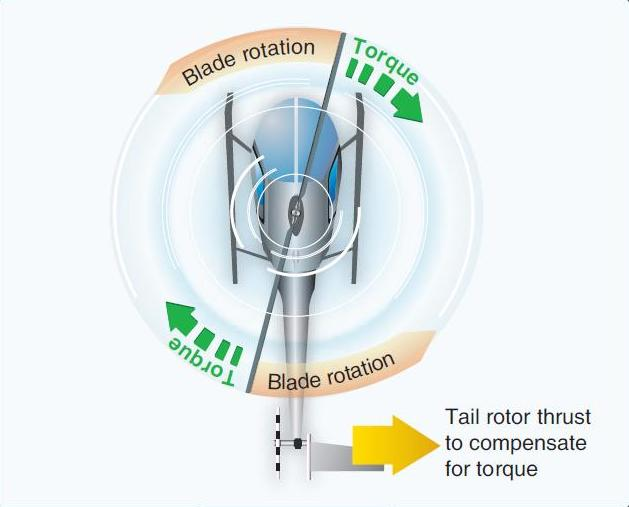
\includegraphics[height = 6cm]{Images/Literature/AntiTorque}
\caption{Image Illustrating generation of Counter Torque (Taken from \cite{Heli})}
\label{IM_Antitorque}
\end{figure}

The capability of any part of a rotor to produce lift is influenced by the local blade position and pressure at that point \cite{Leishman}.
As the rotor spins, the blade's angle of attack shifts. This angle is defined as an azimuth angle ($\psi$) and is measured relative to air flow. The azimuth angle is 0\textdegree down stream and sits at 180\textdegree when it faces directly upstream.
Angular velocity equations state that the speed of any part of the rotor varies along the length of the rotor. With the maximum velocity sitting at the rotor tip. As the rotorcraft adds a horizontal component to its hover or vertical flight, the relative speed of the individual rotor segments now adheres to equation \eqref{EQ_TipSpeed}. As visualised in figure \ref{IM_TipSpeed}, the relative velocity at the any part of the rotor is affected by the azimuth angle of the blade ($\psi$), forward translatory speed of the craft ($V_{\infty}$), angular speed of the rotor ($\Omega$) and the considered distance along the rotor blade (r) \cite{Leishman} \cite{RotorCraftHand}. 

\begin{equation}
\label{EQ_TipSpeed}
V_{r} = \Omega r + V_{\infty}\sin(\psi)
\end{equation}

\begin{figure}[h]
\centering
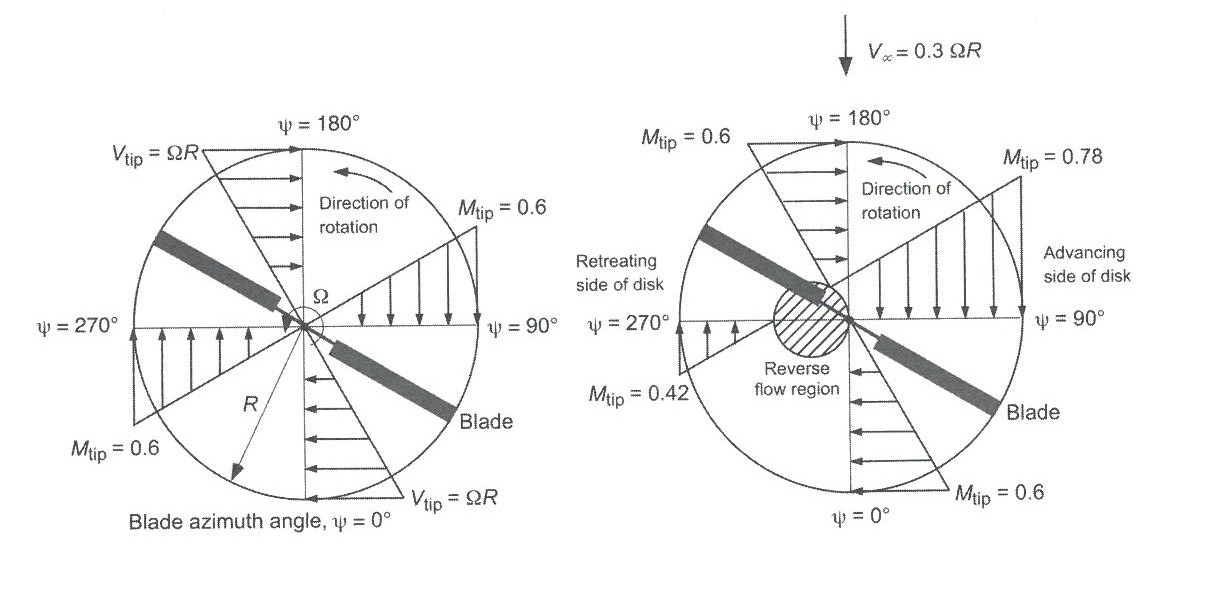
\includegraphics[height = 6cm]{Images/Literature/TipSpeed}
\caption{Velocity components of a rotor \cite{Leishman}}
\label{IM_TipSpeed}
\end{figure}

What this relationship shows is that during forward flight the tip velocity, relative to the ground, changes even if the rotor rotates at a constant speed. This complicates the rotor dynamics at higher speeds and limits the top speed of the craft. On the retreating edge ($\psi = 270$\textdegree $\therefore sin(\psi) = -1$) if $\Omega r <= V_{\infty}$ the rotor would effectively be going backwards and the helicopter is at risk of stalling out, this is known as a stall condition \cite{Leishman} \cite{RotorCraftHand}, while the advancing edge is reaching its maximum speed by approaching Mach conditions and sever instability.

\subsection{Momentum Theory and Thrust Basics}

As mentioned above the rotors of a rotorcraft are responsible for generating all the forces that manoeuvre the vehicle. These forces are induced by pushing air through the rotor disk. With a fixed wing aircraft the analysis of the blades is simplified because the only air flow produced is from the translational velocity of the entire craft. Analysis of blade performance in a rotorcraft can be more challenging as the rotation of the blades must be considered along side the overall speed of the vehicle. As the craft manoeuvres in space, the air flow through the rotor has significant complexities which complicates the analysis. Since the rotorcraft is expected to perform in a variety of flight styles it is important to understand these models, and their flaws. 

To simplify, initially consider a helicopter in a hovering state (Weight(W) = Thrust(T)). Figure \ref{IM_MomentumTheoryAirFlow}, taken from \cite{Leishman}, helps visualise the induced air flow by showing how the rotor smooths out the air by forcing it through the disk area. This more uniform air creates an edge known as the slipstream or wake boundary, with the surrounding air remaining dormant \cite{Leishman}. Inside the wake boundary, the average velocity of the air is tangible and effective, where outside the slipstream edge, the average air velocity is negligible and obsolete. The force required to push that mass of air through the disk space is, by Newton's third law, returned by the air unto the rotor. Thus giving the rotor blades a thrust component.
  
\begin{figure}[h]
\centering
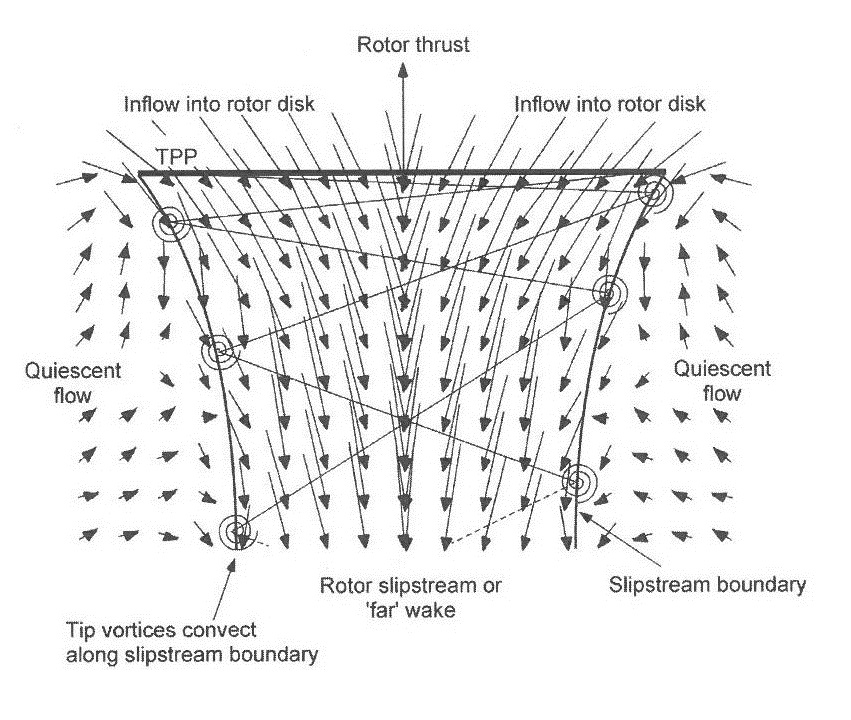
\includegraphics[height = 8cm]{Images/Literature/MomentumTheoryAirFlow}	
\caption{Visualisation of Induced Air Flow Through A Rotor \cite{Leishman}}
\label{IM_MomentumTheoryAirFlow}
\end{figure}

Rankine-Froude's Momentum Theory looks at this induced velocity as well as the displacement of air through the propeller, and attempts to quantify the induced thrust. While figure \ref{IM_MomentumTheoryAirFlow} helps visualise the principle, the variable naming convention for the equations is shown in figure \ref{IM_MomentumTheoryHover} below. 
Labels 0, 1, 2 and $\infty$ refer to the locations of quiescent flow, inflow directly before the rotor, airflow immediately after the disk and the slipstream\footnote{Generally far wake is considered as 1 full rotor diameter distance away \cite{Leishman}.} or far wake condition respectively.
The velocities are shown as the induced velocity in and out the rotor ($v_{i}$), the far wake velocity ($v_{\infty}$) and finally $v_{0}$ represents the zone with zero flow rate. There is no velocity jump across the rotor, the energy being fed into the system by the rotor is represented by a pressure change.

\begin{figure}[h]
\centering
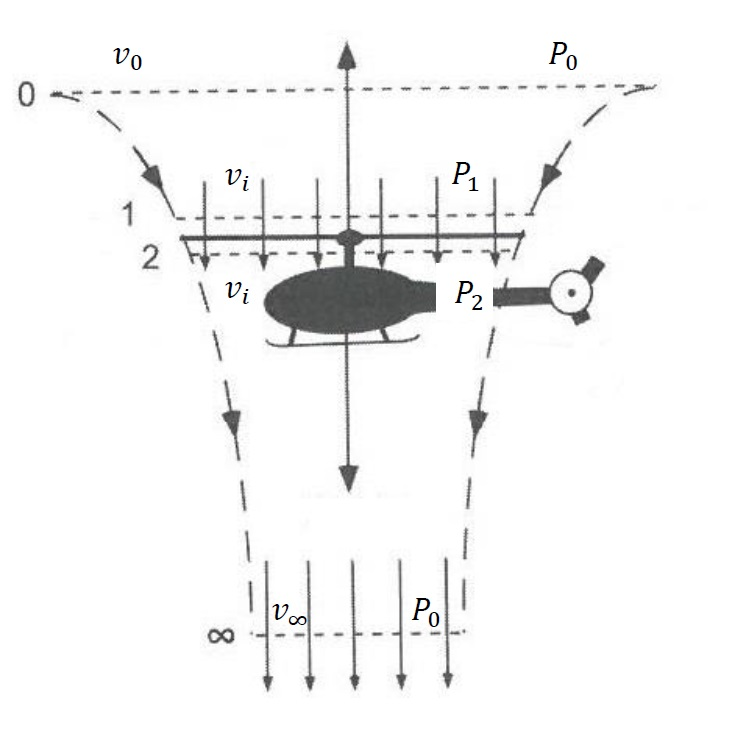
\includegraphics[height = 8cm, angle=360]{Images/Literature/MomentumTheoryHover}			%Must show both air flow as well as far stream and such
\caption{Momentum Theory in Hover (Adapted From \cite{Leishman})}
\label{IM_MomentumTheoryHover}
\end{figure}

As described above, it is by forcing the air through the disk that lift is generated. The mass flow rate of this air can then be described by (\ref{EQ_MassFlow}), where ($\rho$) is the density of air and A is the area of one full blade rotation. The rate at which this mass of air is displaced becomes a crucial variable in rotor dynamics and is directly proportional to thrust (T). This relationship can be quantified as shown in (\ref{EQ_ThrustBasic}). Thrust can also be calculated by finding the difference in pressures over the rotor disk as in (\ref{EQ_ThrustPressure})

\begin{eqnarray}
\dot{m} &=& \rho A v_{i}\label{EQ_MassFlow}\\
T &=& \dot{m}a\label{EQ_ThrustBasic}\\
T &=& A(P_2 - P_1)\label{EQ_ThrustPressure}
\end{eqnarray}

Since $v_0$ is zero during hover and acceleration is the difference in $v_\infty$ and $v_0$, equation (\ref{EQ_ThrustMass}) can be obtained.

\begin{equation}
\label{EQ_ThrustMass}
T = \rho A v_{i} v_\infty
\end{equation}

Thrust can now be quantified if the slipstream and induced velocities are known. 
Then by applying Bernoulli's equation of conservation (\ref{EQ_Bernoulli}) to both sides of the rotor disk, the change in pressure across the disk can be quantified as shown in (\ref{EQ_Bernoulli2}).
That change in pressure fits into one of the initial definitions of thrust (\ref{EQ_ThrustPressure}). Equating both of those definitions yields an important relationship between the three velocities, as shown in (\ref{EQ_RotorVelocity}). The relationship simply states that the induced velocity at the rotor is the average of the quiescent flow above and the far wake velocities. This definition proves useful at a later stage in the rotor theory definitions. 

\begin{equation}
\label{EQ_RotorVelocity}
v_i = \frac{1}{2} (v_\infty + v_0)
\end{equation}

\subsection{Disk and Power Loading}
\subsubsection{Disk Loading}
Disk loading (DL) is a term seen often in the world of rotorcraft, it is a simple but important ratio between thrust and the area a rotating disk makes.  It is represented in its simplest form in the beginning of equation \eqref{EQ_DL}. Since the pressure drop across each rotor is considered uniform, the disk loading for each rotor will equate to the pressure drop across that disk. Equation (\ref{EQ_Bernoulli2}) first shows the difference in pressure and by taking $v_0$ as zero, the second half of equation (\ref{EQ_DL}) can be formed. 
\begin{equation}
\label{EQ_DL}
DL (\frac{N}{m^{2}})= \frac{T}{A} = \frac{1}{2} \rho v_\infty^2
\end{equation}

For multi-rotor craft, the disk loading is assumed uniform across all rotors \cite{Leishman}. The overall disk loading of a single rotorcraft such as a traditional helicopter will be lower than that of a multi-rotor craft of a similar size \cite{RotorCraftHand}.  Figure \ref{IM_DL} shows some examples of disk loading values for a variety of rotor configurations, as shown disk loading is also a measure of hover efficiency.

\begin{figure}[H]
\centering
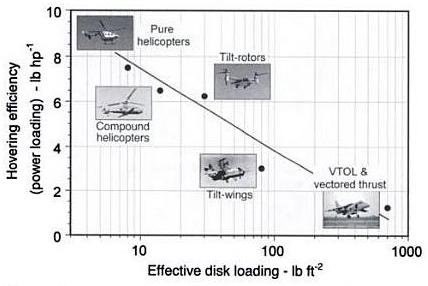
\includegraphics[height = 6cm]{Images/Literature/DL}     
\caption{Image representing, various Disk Loading values for varying rotorcraft (Taken from \cite{Leishman})}
\label{IM_DL}
\end{figure}

A higher disk loading value results in larger values for induced velocities as well as the required power to hover. This means that the larger the blades, the better the efficiency. More force will be generated by pushing large quantities of air slowly, than forcing small amounts of air through at high speeds. Of course with bigger blades, comes larger rotational inertia and geometry as well as the craft being less immune to gusts and interferences. A larger blade also creates faster tip velocities, which will limit the speed of the craft severely \cite{Leishman}.



\subsubsection{Power Loading}
Power is given by the product of both Thrust and the induced velocity at the blade. It can be written as shown in equation (\ref{EQ_Power}). What this ratio shows is that the ideal power is in cubic proportion to the induced velocity at the rotor. Therefore to reduce required power the rotor's induced velocity must be small, which can be accomplished by a significant increase in disk area \cite{Leishman}.

\begin{equation}
\label{EQ_Power}
P = 2 \rho A v_{i}^3
\end{equation}

Another important ratio is between thrust and power, it is called power loading (PL) and is shown in equation (\ref{EQ_PL}). Power loading can be seen as a measure of craft efficiency. 

\begin{equation}
\label{EQ_PL}
PL (\frac{N}{kW})= \frac{T}{P}
\end{equation}

From equations \eqref{EQ_DL} and \eqref{EQ_PL} it can be shown that power loading is inversely proportional to disk loading. Therefore a craft with a lower disk loading will generally be a more efficient platform.

\subsection{Electrical Power to Thrust}
Equation (\ref{EQ_Power}) gives a quantitative approach to solving for aerodynamic power ($P_i$). If electrical power is taken as $P_e = VI$, where V is the applied voltage and I is the sourced current, with an efficiency of $\eta$ then $P_i = \eta VI$. Noting that $P_i = T v_i$ and using equation (\ref{EQ_Power}), a relationship between thrust and $P_e$ can be formed and is represented in equation (\ref{EQ_ElectricalPowerThrust}).

\begin{equation}
\label{EQ_ElectricalPowerThrust}
T = (2\rho A)^{\dfrac{1}{3}} (\eta P_e)^{\dfrac{2}{3}}
\end{equation}

Equation (\ref{EQ_ElectricalPowerThrust}) brings to light a very important relationship which states that thrust grows at a slower rate than the electrical input power to the system.

\begin{equation*}
T \propto P_e^{\dfrac{2}{3}}
\end{equation*}

\section{Analysis of Conventional Rotor Wing Configurations}

Some of the fundamental theories described above relate to the basics behind various rotor configurations and even varying flight techniques. Each different arrangement of blades introduces certain advantages and disadvantages to the system. Not every configuration will be applicable for all operations and it is important to determine what criteria are critical for the intended application.  An analysis of varying rotor configurations is done below and follows a similar trend to that seen in \cite{RotorConfig}, \cite{Bohorquez} and \cite{NewMAV}. The main weighted criterion for the discussion were listed in no particular order as:

\begin{enumerate}
	\item Flight time and efficiency
	\item Geometry and size
	\item Drone Manoeuvrability
	\item Control algorithms
	\item Mechanical complexity
\end{enumerate}

Before the analysis can be done, certain operating parameters of the different craft, surrounding the above mentioned criteria, need to be understood. There has been discussions regarding why and how rotor blades produce lift, this section discusses the real world implementation of those blades.


The same way that a car tyre is the only way the energy from the engine is translated into motion, the rotor in a rotorcraft is responsible for taking the kinetic energy from the motors and translating it into flight. Typically a rotorcraft will be designed with either fixed pitched, or variable pitched rotors. A fixed pitched rotor is a rotor that has an optimally selected, unchangeable pitch and therefore a fixed angle of attack. This of course means that since the angle of attack is fixed for the blade, an increase in speed will be required for a change in lift. With a variable pitched blade, the pilot can change the angle of attack to increase the forces. As the angle of attack increases, the blade will produce more lift without changing the speed of the motor. However, as the pitch increases, so does the drag of the blade. This then requires more motor power to keep the blade moving through the air.
The power requirements for either system are fairly similar, the advantages of a varying pitch is a single rotor has the potential for more dynamic force applications. The downfall however is the high level of complexity in the mechanical design. Both of these facts become pertinent in the final decision making of the platform design.

It is also known that any rotating member will produce a counter rotating torque to the static body, which means that any system with only one rotor will have inherent instability in the yaw axis. The end goal is to have a craft that can fly stably and accurately in 3 dimensions. To do this the craft will need more control surfaces to apply forces in those planes. Figure \ref{IM_PRY}\footnote{http://weboflife.nasa.gov/learningResources/vestibularbrief.htm} shows the planes and the standard naming convention. 

\begin{figure}[H]
	\centering
	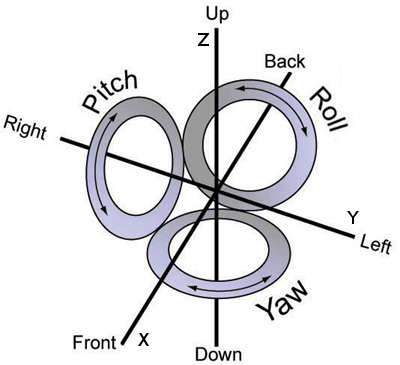
\includegraphics[height = 6cm]{Images/Literature/RollPitchYaw}     
	\caption{Control surfaces required for 3 dimensional flight \cite{Heli})}
	\label{IM_PRY}
\end{figure}

In mathematics discussions are had regarding rotations around the x, y and z axes, in flight theory they are labelled as roll, pitch and yaw. The three axes change as the aircraft changes since they are labelled relative to the aircraft's position. Pitch relates to how much the vehicle is tipping forward or backward, roll is an influence in the left and right rotation, while yaw is rotation around the z axis. Instead of  x, y and z, these axes can be considered as forward, sideways and vertical \cite{Leishman}.

Having only a single, fixed pitched rotor allows only for control in the amount the craft flies up or down, as well as this fore mentioned instability. There are many different methods to obtain full six degrees of flight freedom. The following discussion tries to address each point listed above for each different method, while trying to achieve an optimised design.


\subsection{Helicopter}
When most people think of a rotorcraft they will think of a conventional helicopter, which is still the most widely used configuration for large rotorcraft \cite{RotorConfig}. It consists of a single main rotor, coupled with a smaller counter rotating rotor located in the tail as seen in figure \ref{IM_Helicopter}\footnote{(Adapted from \cite{Heli})}, this is to counteract the developed counter torque as shown in figure \ref{IM_Antitorque}.

\begin{figure}[H]
\centering
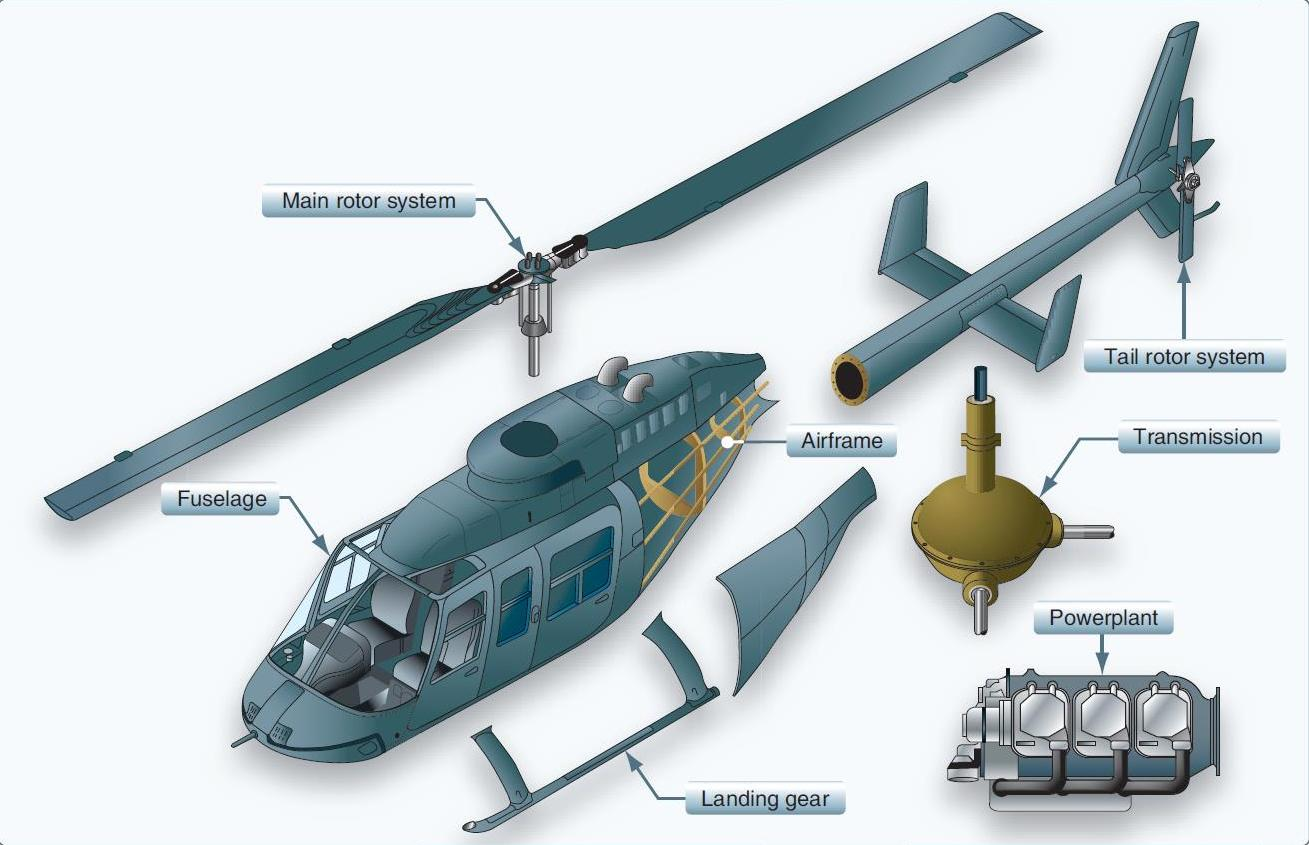
\includegraphics[height = 6cm]{Images/Literature/MainHeliComponents}     
\caption{Main Components of a helicopter \cite{Heli}}
\label{IM_Helicopter}
\end{figure}

The main rotor of a standard helicopter has very low disk loading which gives it excellent hover efficiency. Since the desired end product will mostly be in a state of hover or at least slow lateral movement, this will yield good results for flight time. To achieve yaw stability this configuration makes use of a small tail rotor to counter act the induced moments. The extended tail rotor requires energy which it will draw from the motor while also adding a significant amount of length to the craft. Since the single rotor only gives the pilot thrust control and the tail rotor gives measurable yaw control, there is need for more control surfaces to do more manoeuvring. To implement this most helicopters use a variable pitched rotor system. Cyclic control of this pitch allows the pilot to adjust the angle of attack of the rotor blades while they rotate, thus a forward pitch can be applied by increasing the lift on the left\footnote{This is true for an American style helicopter. The French design requires am increase of lift to the right}. This set up is mechanically very complex and takes intensive control algorithms and laws to give stable control.

Even though the classic helicopter image is always seen as a main rotor with a smaller rotor at the tail, there are many different types of anti torque tail set ups. The ducted fan approach increases the efficiency of the tail rotor by channelling the air flow of the rotor. The NOTAR design \cite{US4200252} as seen in figure \ref{IM_NOTAR}\footnote{(Taken from \cite{Heli})} manipulates the airflow generated by the main rotor and directs it to counter act the induced torque. A tip-jet design eliminates the torque applied to the airframe and therefore no tail rotor is required \cite{RotorConfig}. 

\begin{figure}[H]
\centering
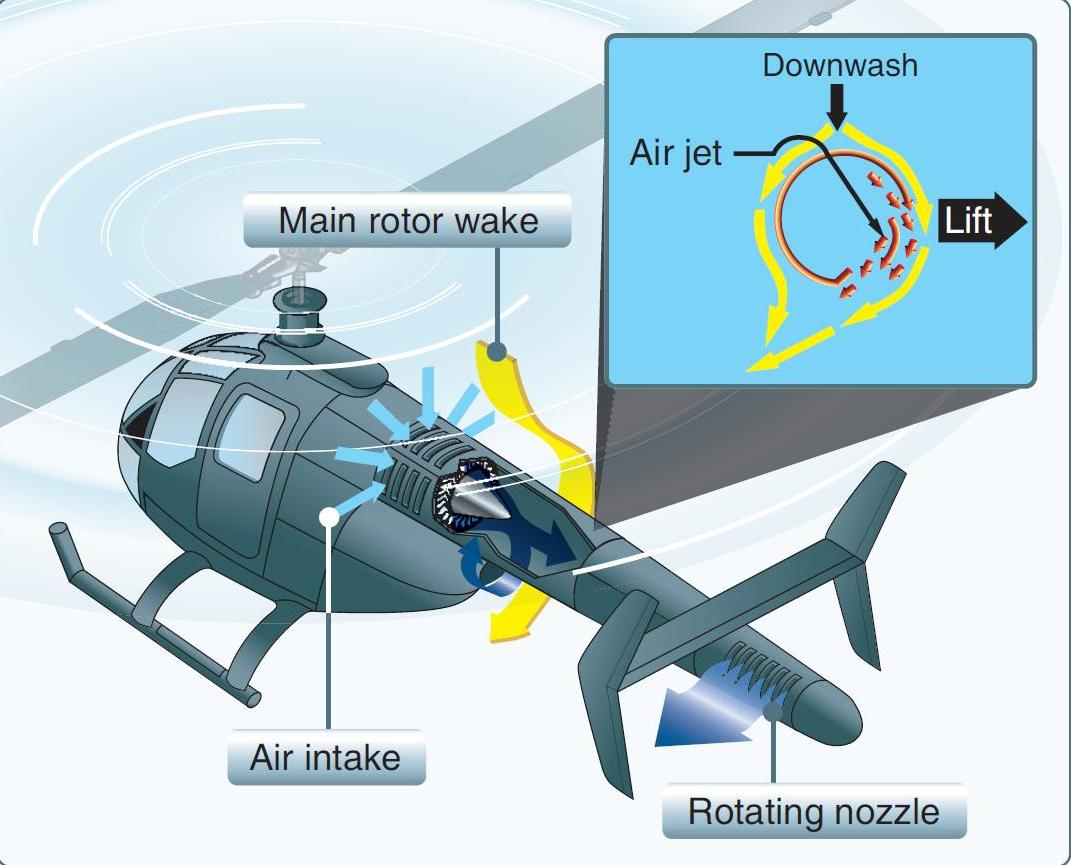
\includegraphics[height = 6cm]{Images/Literature/NOTAR}     
\caption{Image demonstrating the NOTAR system \cite{Heli}}
\label{IM_NOTAR}
\end{figure}

There have been many attempts at improving the standard helicopter design. These improvements have taken the form of adding rotors, designing hybrid aircraft and complex mechanical designs to harvest advantages of both the fixed wing and VTOL craft. Some have even tried to combine multiple features as Flanigan \cite{US7147182} did in his design of a tip-jet, compound, tilt rotor aircraft. 
In an attempt to keep the mechanical complexity to a minimum, not all configurations were investigated.

\subsection{Coaxial Rotors}
A coaxial configuration consists of two counter rotating blades located about the same centre of rotation that both use the same drive system. This eliminates the need for a tail rotor as the torque applied by both rotors cancel each other out, as shown in figure \ref{IM_Coaxial}\footnote{Image Taken from www.simhq.com}.  

\begin{figure}[H]
\centering
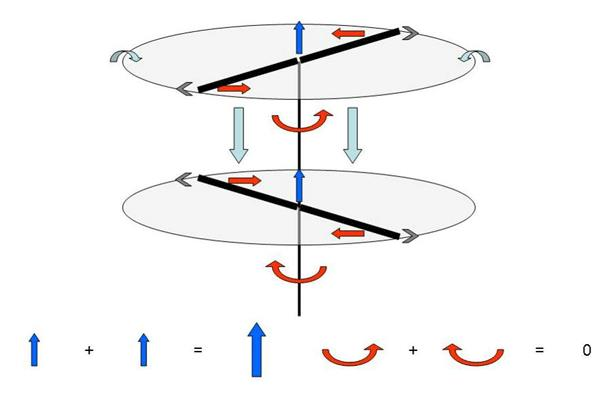
\includegraphics[height = 6cm]{Images/Literature/Coaxial}     
\caption{A standard Coaxial rotor set up and the induced forces}
\label{IM_Coaxial}
\end{figure}

Since half of the bottom blade is working in the top blades slip stream it will have a higher $v_0$ and therefore a larger $v_i$, which according to equation \eqref{EQ_ThrustBasic} will induce a larger thrust, relating to high values of efficiency and disk loading. Localising the blades around a single point also helps with the geometry of the craft as it is a more compact design. With no modifications and only using fixed pitched rotors, this platform will only give yaw and over all thrust control. Bohorquez et al in \cite{Bohorquez} attempted a number of lateral control methods, eventually settling on aerodynamic flaps to control the flow of the downwash, that and other methods are shown in figure \ref{IM_Coaxial_Variations}. Briod et all also used the same set up in his team's design of the Gimball \cite{Briod2012}.
 
\begin{figure}[H]
	\centering
	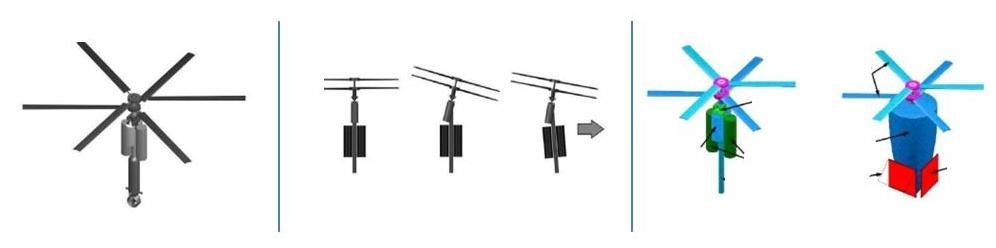
\includegraphics[height = 3cm]{Images/Literature/Coaxial_Configs}     
	\caption{Different methods of lateral control in a Coaxial MAV (Adapted from \cite{Bohorquez})}
	\label{IM_Coaxial_Variations}
\end{figure}

The control flaps are the most common used form of lateral control for small coaxial MAVs. They introduce little mechanical complexity and do not require excessive power to use. The flaps do however decrease efficiency of the system, but if designed correctly should only influence the system while being used. For hover and vertical flight the impact will be negligible. As a control surface the flap is quite rudimentary and will require some more advanced control methods as well as in depth testing to obtain smooth flight transitions. Due to its compactness the design can have considerable manoeuvrability if the control algorithms are designed effectively. Each flap will require an actuator, this will increase total weight, power consumption and required mechanics. 
\todo[inline]{Include Johnson's Calulations that states how much efficeincy is lost due to overlap}

\subsection{Tandem Rotors}

A tandem rotorcraft is sometimes referred to as a dual rotor, as it consists of two blades to generate thrust and to decrease disk loading and increase the lift capacity. In a tandem configuration the blades sit in the front and the rear of the craft, generally with a slight overlap. Tandems are often used in applications that require heavier loads than the traditional rotorcraft can effectively offer. A tandem configuration is demonstrated in figure \ref{IM_Tandem}\footnote{(Taken from \cite{Bee})}, the blades spin in opposite directions to counteract the other one's rotational torque. Pitch and Yaw control are readily available through manipulation of the rotor speeds, while roll control are not as easily accomplished with this design and generally require variable pitch rotors \cite{Oh2005}. Using two smaller blades also decreases the effects of interferences such as gusts on the craft, although a tandem helicopter has the problem of its rear rotor being influenced by the wake of the front rotor\footnote{In the case where the rotors overlap} \cite{Camrad1}. 

\begin{figure}[H]
\centering
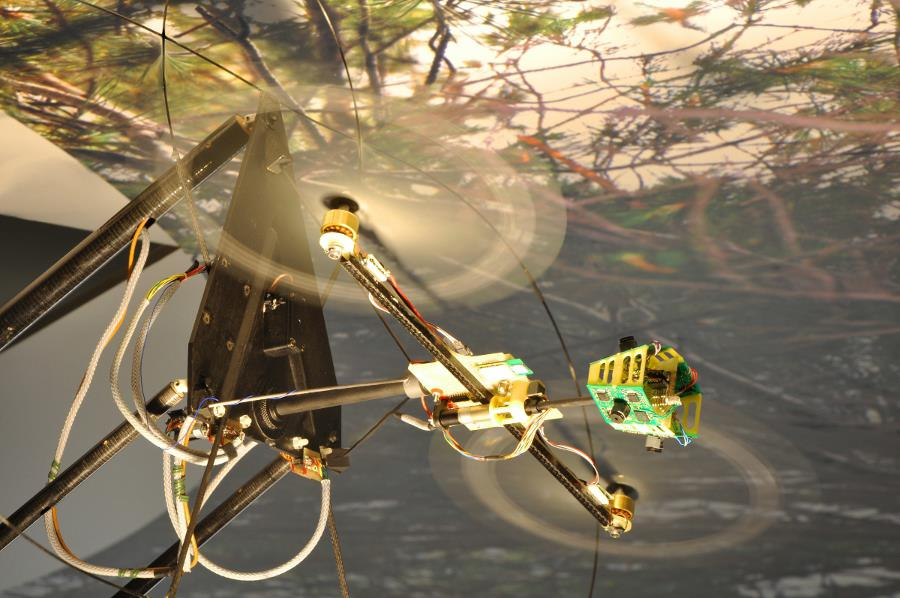
\includegraphics[height = 6cm]{Images/Literature/TandemBEE}     
\caption{The BeeRotor robot demonstrating a Tandem rotor set up in a MAV \cite{Bee}}
\label{IM_Tandem}
\end{figure}


As described in equation \eqref{EQ_ElectricalPowerThrust} the thrust of the system increases slower than the electrical power input into the system. In a standard configuration, doubling the electrical power would only increase the thrust by a factor of $\approx 1.587$. Where as doubling the amount of rotors being driven will double both the thrust and the electrical power. This gives the tandem arrangement the capability of lifting heavier loads with relatively low power consumption, as well as demonstrating low power consumption for hover and slow translatory flight. Having twin blades does increase the size of the craft, but the elimination of the tail rotor sees the size being similar to that of a classic helicopter.


\subsection{Multirotor Designs}

Drones have joined other remote controlled vehicles in the world of hobbyists. Of all the different designs the multirotor is the most popular. Through discussions with drone designers and aerial photographers, the four rotor design is generally chosen due to its incredible stability and manoeuvrability. Similar to the tandem, the quad has very good disk loading and thus can be used to lift heavy loads, there are even products that have 8 rotors to seriously increase the payload capability. This does however relate to a more power hungry system and a less efficient hover.

As shown in figure \ref{IM_CounterBlades}\footnote{(Taken from \cite{ThrustCritical})}, a quad rotor consists of two pairs of counter rotating propellers. Each shaft will be driven by its own motor and unlike the flaps in a coaxial system, every motor in a quadcopter attributes to the lift vector. Having the freedom to control each blade independently gives the pilot advanced manoeuvrability, with minimal mechanical complexities. This also reduces the complexity of the control algorithms as six degrees of freedom can be obtained by simply adjusting the speed of the motors, the multirotor can even rotate on the spot without any change in altitude \cite{ThrustCritical}. Besides the poor hover efficiency, the biggest downside of the multirotor designs is their size and weight. Each blade requires a drive system and space to rotate without interference.

\begin{figure}[H]
\centering
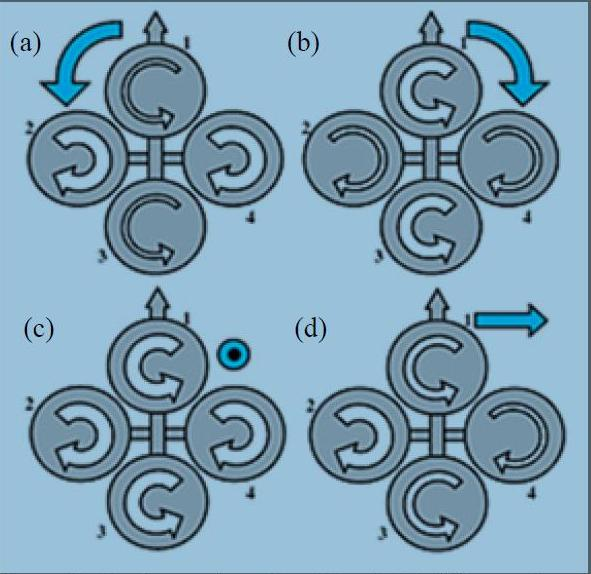
\includegraphics[height =6cm]{Images/Literature/QuadBlades}
\caption{Quadrotor configuration \cite{ThrustCritical}}
\label{IM_CounterBlades}
\end{figure}



\subsection{Tilt Rotors}

A tilt rotor is a very sophisticated system that attempts to harness the benefits of both the fixed and rotor wing aircraft. With the addition of a pivoting axis for each blade the craft has the forward flying speeds of a fixed wing craft while still being able to take off an land vertically like a rotorcraft. The tilt rotor's major downfall is related to the required highly complex and intricate mechanical design \cite{RotorConfig}.
 
VTOL applications require a larger blade to decrease the disk loading, while in forward flight a smaller diameter blade is desired to increase the efficiency of propulsion. Hager \cite{US6030177} developed a telescopic system that transforms the blades to get the optimal benefits out of each configuration, shown in figure \ref{IM_TiltRotor}\footnote{(Taken from \cite{Heli})}. These and other improvements have established the tilt rotor as a  competitive design in the field of aeronautic transportation \cite{RotorConfig}.

\begin{figure}[H]
\centering
\includegraphics[height = 6cm]{Images/Literature/TiltRotor}     
\caption{Hager's design for a telescopic tilt rotor system \cite{Heli}}
\label{IM_TiltRotor}
\end{figure}


\section{Rotorcraft Flight Dynamics}

The flight dynamics of any rotorcraft can be  a complicated problem. This section will discuss some of the methods and issues pertaining to modelling these dynamics. Most of the discussion will surround multirotors, specifically quadrotors, as the majority of the literature is based on these designs \cite{Luukkonen, RealTime, Pounds2006, Hoffmann}. Due to the mechanical complexity of swashplate designs, the discussion is assuming a fixed pitched rotor set up. 

Before control laws can be applied there must be a dynamic model of the craft. To create the model there needs to be a good understanding of the craft dynamics as well as the mathematical methods for creating the appropriate equations. A brief introduction to rigid body dynamics is done and is followed by an in depth talk into modelling rotorcraft for the general case. After the model can be obtained mathematically it is important to discuss the physical implementation of obtaining the data, and the various instrumentation required. Unfortunately its very rare to have a flying environment that is void of disturbances, for this fact the section is ended off with a discussion about the various disturbances that effect the flight dynamics of any rotorcraft.

\subsection{Mass Model and the Inertia Tensor}
In any aerial vehicle mass is always an important design criterion. Every aspect of the platform must be designed to be the lightest it possibly can. Having a light weight craft is one part of the design criterion, another would be ensuring that the weight is geometrically spread out correctly, as well as functionally distributed appropriately. The table below was adapted from \cite{NewMAV} and demonstrates the latter point better. Depending on the different criteria for the craft, different functional blocks will be allocated a certain percentage of weight. For example if the user would like a longer flight time, a higher percentage would be given to the power source and possibly less to the external payload. Generating a good mass model before designing helps better understand the requirements for the craft and could be a deciding factor in the construction.

\begin{table}[H]
\centering
\begin{tabular}{l | c | c | c | c}

Component 					& 0.3kg & 1.8kg & 3.7kg\\
\hline\hline
Rotor System 				& 11.0 & 11.2 & 13.9\\
Tailboom Assembly 		& 8.0 & 9.1 & 7.8\\
Main Rotor Motor 			& 15.4 & 10.5 & 8.1\\
Fuselage/Structure 			& 7.0 &  15.1 & 12.0\\
Main Transmission 			& 2.0 &  3.4 & 3.4\\
Landing Gear 				& 2.3 &  3.4 & 2.9\\
Control System 				& 5.7 & 18.3 & 9.3\\
Avionics 						& 29.4 &  2.4 & 1.6\\
Power Source 				& 19.2 & 26.6 & 41.0\\

\end{tabular}
\caption{MAV Weight Data (Adapted from \cite{NewMAV})}
\end{table}

It was also mentioned that the weight needs to be geometrically positioned correctly, the point of this would be to create as much symmetry in the craft as possible. If this is done correctly the principle axes of inertia will align very closely with the body of the craft, simplifying calculations later on and helping find and define the principle axes. The inertia tensor is a matrix that is a representation of a rigid body's resistance to movements in 3D space, this is obviously crucial since the application is to move a body through 3D space! For the general case the inertia tensor takes the form as shown in equation \eqref{EQ_InertiaTensor}. The inertia tensor is very dependant on a craft's symmetry, and is symmetric itself. In other words, $I_{xy} = I_{yx}$, $I_{xz} = I_{zx}$ and $I_{zy} = I_{yz}$ and therefore if a craft is symmetric about the y axis (x = 0), then $I_{xy} = I_{yx} = 0 = I_{xz} = I_{zx}$ \cite{Luukkonen, MiniFlying}.

\begin{equation}
\label{EQ_InertiaTensor}
\textbf{I} = 
\begin{bmatrix}
I_{xx}	& -I_{xy} & -I_{xz}\\
-I_{yx}	& I_{yy}	& -I_{yz}\\
-I_{zx}	& -I_{zy}	& I_{zz}\\
\end{bmatrix}
\end{equation}


\subsection{Coordinate System}
As mentioned previously, there are six degrees of freedom (DOF) in 3D space, three of them translational and three of them rotational. With a quadcopter, 4 of these degrees of freedom are primary and 2 of them are secondary, being formed by combinations of the primary 4. Generally three dimensional space is modelled in terms of the three orthogonal axes x, y and z; where x and y are lateral movements and the z axis is the vertical movement with gravity being a purely negative z component. These axes will be referred to as the inertial frame and they are relative to the ground and gravity. Now of course the vehicle will not always be perfectly aligned with this frame, for this reason a second frame is defined and refers to the axes that line up with the body of the craft. It is thus named the body frame, these planes will alter as the craft moves around in space. Figure \ref{IM_Frames} visually demonstrates the relationship between the two frames. 

\begin{figure}[H]
\centering
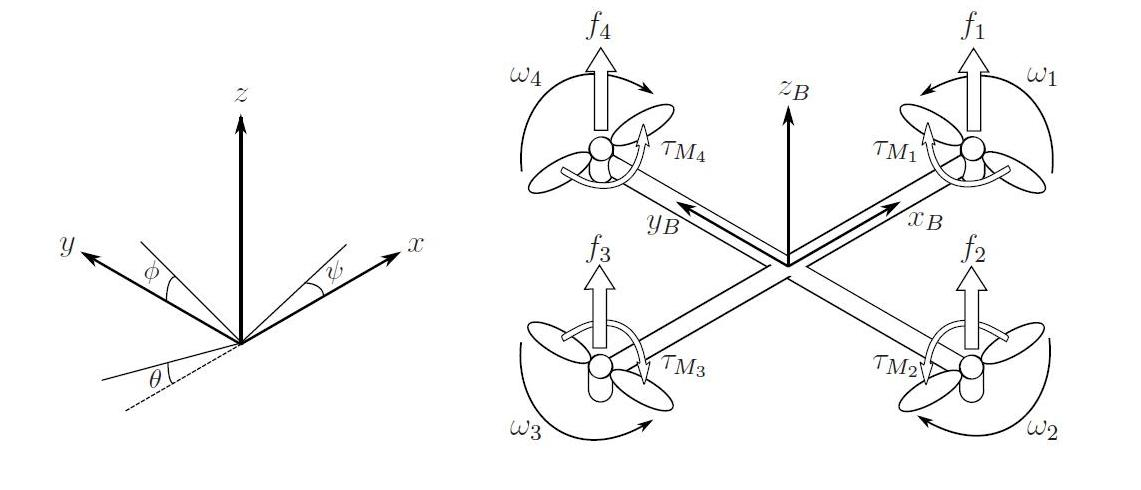
\includegraphics[height = 6cm]{Images/Literature/Frames.jpg}     
\caption{The body and inertial frames of a rotorcraft (Taken from \cite{Luukkonen})}
\label{IM_Frames}
\end{figure}

As shown they are separated by the roll ($\phi$), pitch ($\theta$) and yaw ($\psi$) angles of the craft, which relate to a rotation about the x, y and z axis respectively. These angles are the Euler angles of the rotation and according to Euler's theory, any two varying coordinate axes can be related to one another by a single rotational matrix. In the case of rotating from the body to the inertial frame, the matrix takes the form as shown in equation \eqref{EQ_RotationMatrix} \cite{Luukkonen} where $C_x = \cos(x)$ and $S_x = \sin(x)$. The matrix is also orthogonal, which means that $\textbf{R}^{-1} = \textbf{R}^T$, which would be the rotation from the inertial frame to the body frame \cite{Luukkonen, MiniFlying}.

\begin{equation}
\label{EQ_RotationMatrix}
\textbf{R} = 
\begin{bmatrix}
C_\psi C_\theta   	& C_\psi S_\theta S_\phi - S_\psi C_\phi & C_\psi S_\theta C_\phi + S_\psi S_\phi \\
S_\psi C_\theta   	& S_\psi S_\theta S_\phi + C_\psi C_\phi & S_\psi S_\theta C_\phi - C_\psi S_\phi\\
-S_\theta   		& C_\theta S_\phi & C_\theta C_\phi  \\
\end{bmatrix}
\end{equation}

Therefore if the yaw, roll and pitch angles are known, the angular position of the craft can be calculated with respect to the ground (or the inertial frame). The lateral position will be a combination of x, y and z points in the inertial frame. The naming scheme used in this paper is the same that is seen used by Castillo et al in \cite{MiniFlying, RealTime} with some variations from Luukkonen \cite{Luukkonen} and Carrilo et al \cite{Modelling}. It describes the position of the centre of mass as the value $\boldsymbol{\xi}$ while $\boldsymbol{\eta}$ represents the orientation of the craft in terms of the Euler angles, both numerical representations are shown below. The vector \textbf{\textit{q}} is the culmination of the previous data points to give one complete, descriptive vector for the inertia frame.

\begin{eqnarray}
\boldsymbol{\xi}= 
\begin{bmatrix}
x\\
y\\
z
\end{bmatrix}&
\boldsymbol{\eta} = 
\begin{bmatrix}
\phi\\
\theta\\
\psi
\end{bmatrix}& 
\textbf{\textit{q}} = 
\begin{bmatrix}
\boldsymbol{\xi}\\
\boldsymbol{\eta}
\end{bmatrix}
\label{EQ_InertiaFrame}
\end{eqnarray}

As described above, values in the body frame can be represented in the inertia frame via the rotation matrix $\textbf{R}$, and likewise values in the inertia frame can be represented in the body frame through a rotation of $\textbf{R}^{-1} = \textbf{R}^T$. The body coordinate system takes the same form as the inertia frame, just with a different naming scheme. For simplicity, all vector components relative to the body frame will be followed with a B subscript, so in the inertia frame the components will be the familiar $\hat{\textbf{i}}$, $\hat{\textbf{j}}$ and $\hat{\textbf{k}}$ and the components relative to the body frame will be shown as $\hat{\textbf{i}}_B$, $\hat{\textbf{j}_B}$ and $\hat{\textbf{k}}_B$.

It makes sense that the global position and orientation of the craft be described in the inertia frame, since generally those values will be discussed relative to that frame. The velocities however will generally be discussed relative to the body frame. Since there is now a simple relationship between the two frames, it is possible to assess different parameters in the different frames, as long as when they are discussed together they are both converted to the same coordinate axes. Equation \eqref{EQ_BodyFrameSpeeds} represents the translational speeds as $\textbf{V}_B$ and the rotational speeds as $\boldsymbol{\Omega}_B$, both of which are relative to the body frame.

\begin{eqnarray}
\textbf{V}_B = 
\begin{bmatrix}
V_{x_B}\\
V_{y_B}\\
V_{z_B}
\end{bmatrix}&
\boldsymbol{\Omega}_B = 
\begin{bmatrix}
p\\
q\\
r
\end{bmatrix}
\label{EQ_BodyFrameSpeeds}
\end{eqnarray}

Rotation matrix $\textbf{R}$ is used to describe variables measured in the body frame to the inertia frame. As seen in Luukkonen \cite{Luukkonen} the general case for velocities will require a rotation from the inertial frame to the body frame. That is done with a rotation $\textbf{\textit{W}}_\eta$, with the inverse being a rotation for speeds taken in the body frame to the inertial frame. Therefore $\boldsymbol{\Omega}_B = \textbf{\textit{W}}_\eta \times \dot{\boldsymbol{\eta}}$ and $\dot{\boldsymbol{\eta}} = {\textbf{\textit{W}}_\eta}^{-1} \times \boldsymbol{\Omega}_B$. Where $\textbf{\textit{W}}_\eta$ is represented by the matrix shown in equation \ref{EQ_VelocityRotation} \cite{Luukkonen, Modelling}.

\begin{equation}
{\textbf{\textit{W}}_\eta} = 
\begin{bmatrix}
1 & 0 & -S_\theta\\
0 & C_\phi & C_\theta S_\phi\\
0 & -S_\theta & C_\theta C_\phi
\end{bmatrix}
\label{EQ_VelocityRotation}
\end{equation}

In summation, the local coordinates of the craft will be measured according to the inertial axes and can be translated to the body frame through the rotation $\textbf{R}$. The coordinates are represented by the variable $\textbf{\textit{q}}$. Which encompasses the lateral position ($\boldsymbol{\xi}$) and the rotational position, or orientation, ($\boldsymbol{\eta}$).The velocities of the craft however, will be measured relative to the body frame and can be converted to the inertial frame using the rotation $\textbf{\textit{W}}_\eta$. The velocities are also composed of translational ($\textbf{V}_B$) as well as rotational components ($\boldsymbol{\Omega}_B$).

\subsection{Dynamic Flight Model}

The general coordinates of a system, like the ones described above, is the smallest set of parameters that can unambiguously describe the configuration of that system. The number of variables used will equal to the number of degrees of freedom \cite{MIT}. 
Since the vector \textbf{\textit{q}} gives an absolute position of the craft, the derivative, $\dot{\textbf{\textit{q}}}$, should represent the speeds with the double derivative, $\ddot{\textbf{\textit{q}}}$, giving accelerations. The form of the problem allows the use of Lagrangian mechanics and formulae to solve for the forces \cite{MIT, MiniFlying}. Since the system can be considered as  a rigid body, normal Newtonian mechanics can be used to solve the problem and will also use the Euler angles described above \cite{Luukkonen, Modelling}. Both methods are briefly discussed, using a standard quadcopter as an example. Before the models can be generated a discussion must be had on the forces involved.  Figure \ref{IM_Frames} is used as a descriptive aid for the following section.


\subsubsection{Translational Forces}
For a quadcopter all the forces are generated by the 4 rotors. Simplifying the system that the rotors are fixed-pitched entails that the applied forces only have a tangible $\hat{\textbf{k}}_B$ component.

\begin{eqnarray}
\textbf{F}_B = (f_1 + f_2 + f_3 + f_4)\hat{\textbf{k}}_B & where & f_i = k_i {\omega_i}^2
\label{EQ_Translational}
\end{eqnarray}

The individual force components ($f_i$) can be calculated using a constant ($k_i$) and the angular rotor speed ($\omega_i$) \cite{RealTime}. Now that the forces are expressed in the body frame, they can be converted into the inertial frame through the rotation $R^T$. Therefore $\textbf{F}_\xi = R^T \textbf{F}_B$.

\subsubsection{Rotational Forces}
As said above, all of the controlled forces are generated by the rotors, this includes the moments. The traditional variations in angular position that the quadcopter experiences are all created by independently varying the speed of the motors. These moments can be mathematically expressed as shown in \ref{EQ_moments}, $l$ is the distance from the centre of the rotor to the centre of gravity. \cite{Modelling}

\begin{eqnarray}
\tau_\psi = \sum_{1}^{4} \tau_{M_i};&
\tau_\theta = (f_2 - f_4)l_{4,2};&
\tau_\phi = (f_3 - f_1)l_{1,3}
\label{EQ_moments}
\end{eqnarray}

Effectively what the equations say is that if a there is an imbalance in the clockwise and counter-clockwise rotations, there will be an induced yaw moment ($\tau_\psi$). If differential commands are sent to geometrically opposite rotors, there will either be an induced pitch ($\tau_\theta$) or roll ($\tau_\phi$) moment, depending on how the frames are set up, this is demonstrated in figure \ref{IM_CounterBlades}.

\subsubsection{Accelerations Model}
Equations \ref{EQ_Translational} and \ref{EQ_moments} refer to the input forces, or control authority we have. To complete the model it is necessary to now understand how these inputs effect our global position \textbf{\textit{q}}. Using the Lagrangian in equation \ref{EQ_Lagrange} accelerations in the six DOF  can be solved for. Equation \ref{EQ_LagrangeAcceleration} shows the result of this mathematics and completes the model used by Castillo et al \cite{MiniFlying, RealTime}. Each output, or degree of freedom, is now related to one of the input forces.

\begin{eqnarray}
\label{EQ_LagrangeAcceleration}
m\ddot{x} &=& -\lvert \textbf{F}_B \rvert\sin\theta\\
m\ddot{y} &=& \lvert \textbf{F}_B \rvert\cos\theta\sin\phi\\
m\ddot{z} &=& \lvert \textbf{F}_B \rvert\cos\theta\cos\phi - mg\\
\ddot{\psi} &=& \tilde{\tau}_\psi\\
\ddot{\theta} &=& \tilde{\tau}_\theta\\
\ddot{\phi} &=& \tilde{\tau}_\phi
\end{eqnarray}

Although Castillo's model has obtained some positive results, his model is simplified with decisions such as neglecting the Coriolis effects from the rotors. This simplification can be seen by the addition of the tilde above the torque symbols in \ref{EQ_LagrangeAcceleration} and  can be seen in numerous readings \cite{MiniFlying, RealTime, Modelling}. Even with these faults the model is a good basis for modelling a rotorcraft. Luukkonen in \cite{Luukkonen} decided not to neglect the Coriolis effects and added an additional term into his model, $\textbf{C}(\boldsymbol{\eta}, \dot{\boldsymbol{\eta}})$, which is a three by three matrix holding all the Coriolis values. 

\begin{eqnarray}
\label{EQ_LagrangeAccelerationCoriolis}
\boldsymbol{\tau} = \textbf{C}(\boldsymbol{\eta}, \dot{\boldsymbol{\eta}})\dot{\boldsymbol{\eta}} + \mathbb{J}\tilde{\boldsymbol{\tau}} & where & \tilde{\boldsymbol{\tau}} = \begin{bmatrix}
\tilde{\tau}_\phi\\
\tilde{\tau}_\theta\\
\tilde{\tau}_\psi
\end{bmatrix}
\end{eqnarray}


\subsubsection{Euler-Lagrangian Approach}
The Lagrange model is repeatedly used in generating models for rigid body dynamics \cite{MIT, MiniFlying, Luukkonen, RealTime}. There are a few benefits to using this model opposed to the standard Newtonian approach. The Lagrange approach produces as many equations as their are degrees of freedom, in a system where there are 6 degrees of freedom this can become pertinent to solving the model. Using the Lagrangian automatically eliminates non-contributing forces and it will take advantage of the now formulated general coordinate system described above \cite{MIT}.

The Lagrangian uses the energy conversation principles to obtain a formula for the forces acting in a system. The Lagrangian function is the difference between the kinetic (\textbf{T}) and potential energies (\textbf{U}), it takes it simplest form as $ \textbf{L}( \textbf{\textit{q}}, \ddot{ \textbf{\textit{q}}}) = \textbf{T} - \textbf{U}$, equation \eqref{EQ_Lagrange} is the expanded equation. 
Where the kinetic energy is broken into two parts, rotational and translational. The major contributing potential energy takes the form of $\textbf{U} = (mgz) \hat{\textbf{k}}$ and it represents the gravitational potential of the craft. The kinetic energies can be represented as $\textbf{T}_{rot} = \dfrac{1}{2} \dot{\boldsymbol{\eta}}^T \mathbb{J} \dot{\boldsymbol{\eta}}$ and $\textbf{T}_{trans} = \dfrac{m}{2} \dot{\boldsymbol{\xi}}^T \dot{\boldsymbol{\xi}}$. Where $\mathbb{J}$ is the inertia tensor in terms of $\boldsymbol{\eta}$ and $\mathbb{J} = {\textbf{\textit{W}}_\eta}^T \textbf{I} \textbf{\textit{W}}_\eta$ \cite{Luukkonen, Modelling}.

\begin{eqnarray}
\textbf{L}( \textbf{\textit{q}}, \ddot{\textbf{\textit{q}}}) =  \dfrac{1}{2} \dot{\boldsymbol{\eta}}^T \mathbb{J} \dot{\boldsymbol{\eta}} + \dfrac{m}{2} \dot{\boldsymbol{\xi}}^T \dot{\boldsymbol{\xi}} - mgz
\label{EQ_Lagrange}
\end{eqnarray}

The actual model is then based on the standard form of the Euler-Lagrange equations is shown in equation \eqref{EQ_EulerLagrange} below.

\begin{equation}
\dfrac{d}{dt} \dfrac{\partial \textbf{L}}{\partial \dot{\textbf{\textit{q}}}} -  \dfrac{\partial \textbf{L}}{\partial \textbf{\textit{q}}}= \textbf{F}
\label{EQ_EulerLagrange}
\end{equation}

Where $\textbf{F}$ is the culmination of all the forces being experienced by the craft in relation to the inertial frame. Since the Lagrangian accounts for all the degrees of freedom, $\textbf{F}$ encompasses both the translational forces ($\textbf{F}_\xi$) as well as the rotational moments ($\boldsymbol{\tau}$), $\textbf{F} = (\textbf{F}_\xi, \boldsymbol{\tau})$. It can be seen from equation \eqref{EQ_Lagrange} that these two forces can be observed independently from each other \cite{RealTime}.

\subsubsection{Newton-Euler Method}
The method described above involves using the Lagrangian definition to obtain the equations of motion. Another method is to keep the same coordinate system using Euler's methods and then applying Newton's laws of motion to obtain the model. Either approach will yield a model and will depend on personal preference for a decision. Newton's method is more familiar to some and does not involve the more complicated Lagrangian mathematics. The downfall is the coordinate system derived above is not fully taken advantage of, and the mathematical model can feel more complicated since non-contributing forces are still considered. The Newton model does however allow elimination of certain disturbances due to referencing from different frames. 
In \cite{Luukkonen, Modelling} both approaches are analysed an compared and it is shown that both approaches obtain the same model.

When using the Newton-Euler method, it is of crucial importance to remember which reference frame is being worked with. Ideally an absolute value for accelerations is desired i.e using the inertial frame as a reference. To begin, consider the forces required to accelerate the mass $m\textbf{V}_B$ as well as to counter the centrifugal force $\boldsymbol{\Omega}_B \times (m\textbf{V}_B)$. These forces take the form of the applied thrust $\textbf{F}_B$ as well as the gravity component, a rotation is needed to place the gravitational force in the body frame resulting in a force of $\textbf{R}^T \textbf{G}$ \cite{Luukkonen}. Relating these via Newton's 2nd law of motion, \eqref{EQ_EulerNewton} can be obtained.

\begin{equation}
m\textbf{V}_B + \boldsymbol{\Omega}_B \times (m\textbf{V}_B) = \textbf{F}_B + \textbf{R}^T \textbf{G}
\label{EQ_EulerNewton}
\end{equation}

Since centrifugal forces are eliminated when using the inertial frame, \eqref{EQ_EulerNewton} can be used to obtain  \eqref{EQ_EulerNewtonInertial} which can also be represented in matrix notation, as shown in \eqref{EQ_EulerNewtonInertialMatrix} \cite{Luukkonen}. 

\begin{equation}
m\ddot{\xi}  = \textbf{R}\textbf{F}_B + \textbf{G}
\label{EQ_EulerNewtonInertial}
\end{equation}

\begin{equation}
\begin{bmatrix} \ddot{x}\\ \ddot{y}\\ \ddot{z} \end{bmatrix} = -g\begin{bmatrix} 0\\ 0\\ 1 \end{bmatrix} + \frac{\textbf{F}_B}{m} \begin{bmatrix}
C_\psi S_\theta C_\phi + S_\psi S_\phi\\
S_\psi S_\theta C_\phi - C_\psi S_\phi\\
C_\theta C_\phi
\end{bmatrix}
\label{EQ_EulerNewtonInertialMatrix}
\end{equation}

As for the rotational velocities, the external torque ($\boldsymbol{\tau}$) must be big enough to provide the inertia ($\textbf{I}$) with the required acceleration ($\boldsymbol{\dot{\Omega}}_B$), while overcoming the centripetal ($\boldsymbol{\Omega}_B \times \textbf{I}\boldsymbol{\Omega}_B$) and the gyroscopic forces ($\boldsymbol{\Gamma}$). Equation \eqref{EQ_EulerNewtonRotation} is the mathematical representation of the applied torque. Equation \eqref{EQ_EulerNewtonRotationMatrix} is the matrix where the accelerations have been solved for.

\begin{equation}
\textbf{I} {\boldsymbol{\dot{\Omega}_B}} + \boldsymbol{\Omega}_B \times \textbf{I}\boldsymbol{\Omega}_B + \boldsymbol{\Gamma} = \boldsymbol{\tau}
\label{EQ_EulerNewtonRotation}
\end{equation}

\begin{equation}
\begin{bmatrix}\dot{p}\\ \dot{q} \\ \dot{r} \end{bmatrix} = \begin{bmatrix} I_{yy} - I_{zz}qr/I_{xx}\\ I_{zz} - I_{xx}pr/I_{yy}\\ I_{xx} - I_{yy}pq/I_{zz} \end{bmatrix} - I_r \begin{bmatrix} q/I_{xx}\\ -p/I_{yy} \\ 0 \end{bmatrix} \omega_\Gamma + \begin{bmatrix}\tau_\phi/I_{xx} \\ \tau_\theta/I_{yy} \\ \tau_\psi/I_{zz}  \end{bmatrix}
\label{EQ_EulerNewtonRotationMatrix}
\end{equation}

Where $\omega_\Gamma = \omega_1 - \omega_2 + \omega_3 - \omega_4$ \cite{Luukkonen}.

\subsection{Disturbances}
The acceleration model developed by Castillo et al \cite{MiniFlying} only considers forces generated by pilot inputs to the system. Most readings that involve rotor dynamics will include a section about disturbances, or aerodynamic effects \cite{Hoffmann, Pounds2006, Luukkonen, NearWall} since they also can severely effect the craft dynamics. Most of the aerodynamic forces are only pertinent at higher velocities, as they are created through an increase in velocity of the air speed. In the case of Luukkonen \cite{Luukkonen}, he addresses the disturbances but omits them from the model since they are negligible at the speeds his craft would be travelling.

\subsubsection{Drag}
Drag is a resistive force whose quantity is relative to the speed of the object in question and is always in the direction opposing the motion. It can be seen as the friction forces created by the air. Equation \ref{EQ_Drag} quantifies the effect of drag. Luukkonen \cite{Luukkonen} uses a simple matrix to include the drag effects in his acceleration model, simply subtracting the components of drag from each acceleration component. As seen from the equation, the effect of drag can be reduced through mechanical design, by reducing the area of the plane facing towards the direction of the motion. 

Since the rotors spin at such high speeds they also experience high levels of drag, the effect of rotor drag is seen as a drop in efficiency as it constantly acts against the motors. Rotor drag is also responsible for other random disturbances in the craft dynamics.

\subsubsection{Blade Flapping}
It was mentioned earlier in the text about the issue with the difference in tip velocities for the advancing and the retreating case. Not only is it a total speed limitation, it also creates a disturbance called blade flapping. Figure \ref{IM_BladeFlapping}\footnote{Taken from (http://www.dynamicflight.com/aerodynamics/flapping/) and \cite{Hoffmann}} shows two different views of the effect as a visual aid in this subsection. 

The difference in velocity of the two edges creates a cyclical variance in angle of attack, similar to an uncontrolled version of cyclic control used in the traditional helicopter. This varying angle of attack creates a dissymmetry of lift that causes instability in the craft and a flapping motion of the rotors. The blades will flap up and down in a single revolution creating a very fast disturbance equations, for this reason they can be seen as instantaneous functions, and the timing of the flapping does not need to be considered \cite{Pounds2006}.

As described in \cite{Hoffmann, Pounds2006}, this variance in angle of attack effectively creates a new frame which lines up with the now angled rotors. Angle $a_{1s}$ is the deflection from the rotor normal and is the modification variable of the of thrust components. This results in a decrease in the $\hat{\textbf{\textit{k}}}_B$ component of thrust equivalent to $\cos (a_{1s})$. The lateral component of this force is cancelled out by the symmetry of the quadcopter, as well as the moment it produces around the rotor \cite{Hoffmann}.

\begin{figure}[H]
\centering
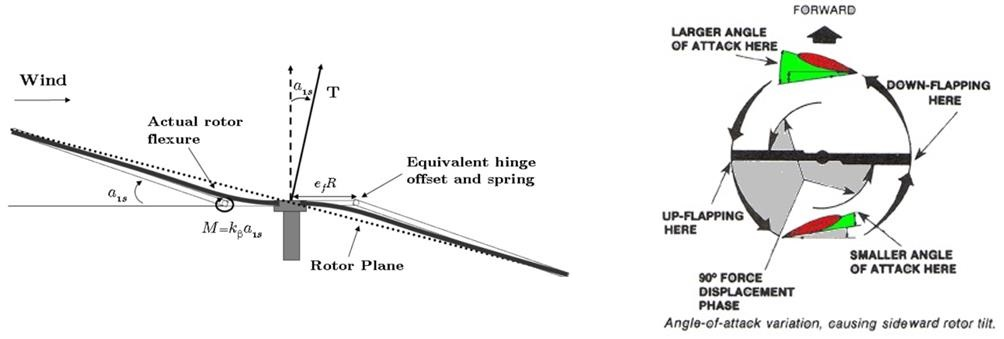
\includegraphics[height = 5cm]{Images/Literature/BladeFlapping3}     
\caption{Qualitative effects of blade flapping.}
\label{IM_BladeFlapping}
\end{figure}

Blade flapping will not be apparent when the craft is in a state of hover and there is no wind. Flying the quadcopter effectively generates wind lateral to the rotors and this causes the change in speeds of the rotor tips. The problem is generated by the non zero airflow through the rotors. Airflow disruption in general will cause quantifiable effects to the rotorcraft and should definitely be included in the model.

\subsubsection{Airflow Disruption}
Airflow can be an ambiguous phrase, since it is not always the air that is flowing, rather it could be labelled as relative airflow since that is what affects the dynamics of the craft. Airflow can be seen as the stream of air from $v_0$ to $v_i$ and then all the way down to $v_\infty$ similar to that shown in in figure \ref{IM_MomentumTheoryAirFlow} with naming scheme following figure \ref{IM_MomentumTheoryHover}. The three velocities are all linked through equation \ref{EQ_RotorVelocity} and equation \ref{EQ_ThrustMass} states that thrust is directly proportional to these velocities. It can be shown then that any deviation in these velocities will vary the thrust of the rotor in question. $v_0$ is only zero when the craft is in a state of pure hover, completely stationary, and there is no wind. Increasing the speed of the craft will increase the $v_0$ component creating a variation in the overall thrust, the same can be said for any condition that contains a tangible wind factor. 

Humidity and air density also play a significant role in rotor dynamics, although it is very unlikely that the air percentages will suddenly change, this must be considered when designing a craft for multiple climates and seasons.

The third airflow disruption that will be addressed is the effects that mechanical intrusions will have on the far wake velocity. In the design of STARMAC by Hoffmann et al \cite{Hoffmann} the frame was designed to be very configurable so that the effects of the mechanical design could be quantified. Originally the rotors were shrouded and quite close to the COG of the craft. The shrouds were a distance of 5\% rotor radius and when removed the yaw tracking improved from $\pm$10\textdegree to $\pm$3\textdegree. When not included in the dynamic model the obstruction in the air stream will cause lower and less stable values of thrust, affecting the stability of the model. 
When the rotors were located close to the centre of gravity they obtained some attitude disturbances that were eliminated by moving the rotors further away. It was also observed that any object that lies close to the rotor tip, created intense arbitrary disturbances and should be avoided. 

There is another disturbance that greatly affects the rotor performance called near ground or near wall effect and as the name stipulates, only occurs when the craft approaches a large immovable object.

\subsubsection{Near Ground Effect} \label{SSSECT_NearGroundEffect}
Robinson et al \cite{NearWall} created and validated a computational fluid dynamics mode to help quantify and understand the effects of near wall hovering for a traditional micro helicopter. The results of the study mainly focus on the rotor and thus will be very applicable to a collision resistant MAV regardless of the rotor configuration.

Figure \ref{IM_NearWall} is an image generated through the model and represents the velocities of the air stream descried above. Note how the no wall case represents, very closely the air flow described in figure \ref{IM_MomentumTheoryAirFlow} while the near wall case has some deviations. Effectively the velocities close to the wall are significantly less uniform than those that are away from the wall. This phenomenon is caused by the boundary layer created close to the wall. This asymmetry in the induced air stream creates reaction forces, the magnitude of which changes as the azimuth angle of the rotor changes. Since the rotors spin at such high velocities the force can be averaged to get a force component that only has tangible effects in the direction of the wall. The component parallel to the wall is not greatly affected as there is still a considerable amount of symmetry in that direction. Due to these reaction forces there is an induced moment that will reduce gradually as the rotor gets further away from the wall.  

\begin{figure}[H]
\centering
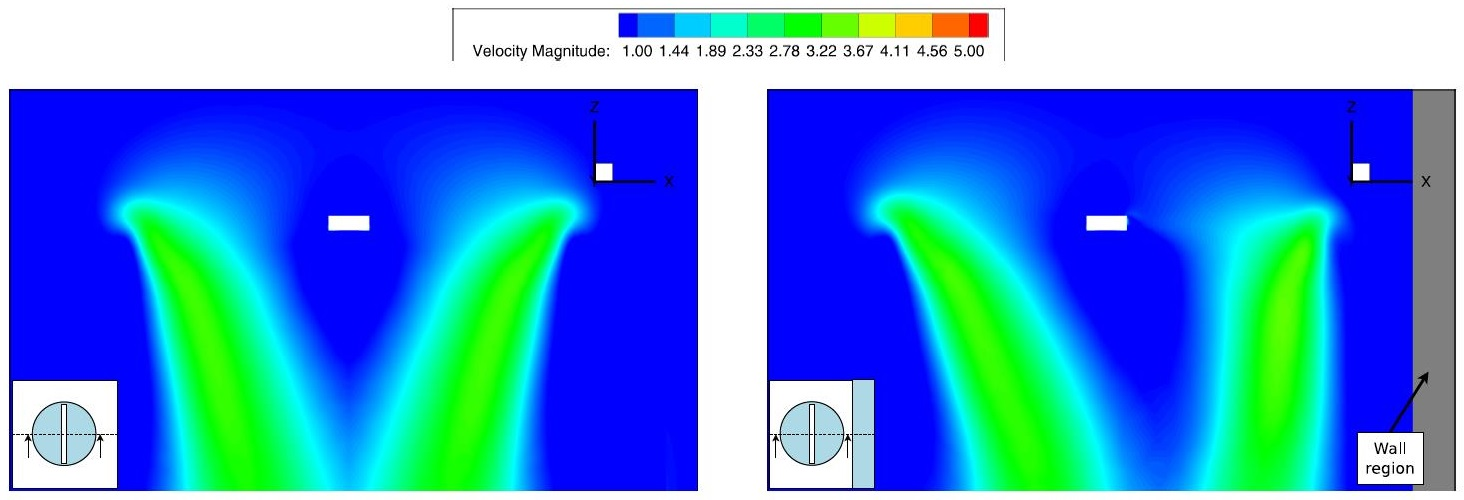
\includegraphics[height = 5cm]{Images/Literature/NearWall}     
\caption{Velocity components though the rotor for, no wall (left) and near wall (right) conditions (Taken from \cite{NearWall})}
\label{IM_NearWall}
\end{figure}

In \cite{NearWall}, Robinson et al used the script $c$ as their unit of measure for distance to the wall, $c$ is chord length of the airfoil. The graph shown in Figure \ref{IM_NearWallGraph} shows how the moment felt by the craft varies with the distance to the wall.

\begin{figure}[H]
\centering
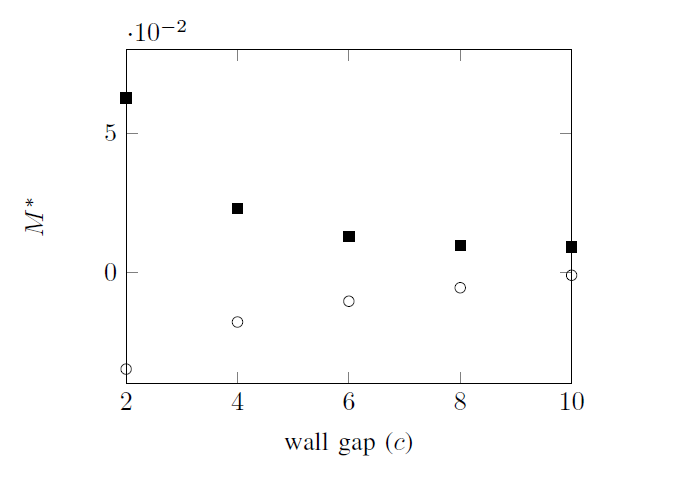
\includegraphics[height = 5cm]{Images/Literature/NearWallGraph}     
\caption{Graph showing relationship between distance from the wall and moment felt be the craft (Taken from \cite{NearWall})}
\label{IM_NearWallGraph}
\end{figure}

In \cite{NearWall} they conclude their paper by describing a proposed method of control which will be discussed further in the text.

\subsection{Instrumentation}
\todo[inline]{Incomplete}
In the final chapter of the book written by Castillo et al \cite{MiniFlying} there is a section on appropriate instrumentation for use in a MAV. The chapter includes devices such as a GPS and various other sensors and microcontrollers that can be added to a rotorcraft design. This section of the report will only address sensors that will aid in attitude and other movement measurements.

The most commonly used


\section{Methods for Control}
\todo[inline]{Incomplete}
\subsection{Stable Hover}
\subsection{Altitude Control}
\subsection{Attitude Control}
\subsubsection{Disturbance Observer}
\todo[inline]{\cite{NearWall} has awesome section on this}

\section{Collision Protection Techniques}
\todo[inline]{Need to decide if I should keep this in,l and in what format}
\cite{Klaptocz2013, Collision, Klaptocz2012, Briod2012, Daler2013, Klaptocz2010}
\subsection{Collision Avoidance}
%Not suitable for this application will still include some collision avoidance techniques
\subsection{Impact Resistance}
%Refer to impulse equations, Newtons's laws
%look at car designs
Impact resistance is a technique used by a variety of fields in the world today. Included in this is something as simple as the shocks or suspension in a car, they are designed to allow the automotive to withstand sudden impacts. Generally these techniques use a component that has some tangible spring constant.


\subsection{Rolling Cage}
\todo[inline]{Although a lot can be learnt from this design in terms of collision resistance, for the proposed end use case the design will not be pursued. The rolling cage design}
\chapter{System Requirements}
This chapter sets to lay out as an introduction to the research. By discussing the end use case of the design, a few critical research questions can be raised. A problem statement will be drawn out by these questions. The chapter will then be concluded with a list of extracted requirements that the system needs to address and ultimately accomplish. \todo{Needs editing}

	\section{Background}
	Tracked and wheeled robots are beginning to reach their limitations, and society is in need of more complex and versatile vehicles. For a land robot to successfully navigate an extremely complex or cluttered environment, the designer must look at creating a legged robot. Legged designs introduce complexity into any system due to the intensive control theory required. There has been some great progress in legged designs, such as Big Dog created by Boston Dynamics \cite{BigDog}. Nevertheless, deploying currently available legged platforms could cost valuable time with lengthy navigation routines. An alternative approach would be to use an aerial platform that could do overhead surveillance. A drone could complete the required task by flying over the complexities in the operating environment. However, with conventional flight techniques and platforms, almost any sort of collision would cause a failure and the system would not be able to complete its mission. This limits this approach to only work in a situation where the drone would be able to fly over the obstacles. 

	Unfortunately, many of the desired use cases are not open aired and the platform will be required to fly below and even through obstacles to complete its task. A good example of this is in search and rescue missions. An aerial vehicle will be required to navigate through damaged or even collapsed buildings. The same platform could be used in a mining environment. Used to assist miners in assessing unexplored and potentially dangerous areas. 
	From the late 1800s South Africa has had a massive mining community, with coal, gold and diamond mining being used as a major source of income and job creation for the country. In response to this, two South African research institutes have agreed to a joint collaboration in solving some of these aspects for an underground mine environment. This project involves both The University of Stellenbosch (US) and the Council of Scientific and Industrial research (CSIR). A mining environment has many applications for a collision resistant drone. Such as the mapping of unknown and potentially hazardous environments. The drone would be able to fly in, conduct a survey of the environment and feed that information back to the miners, ensuring a safer work environment while minimising costly delays. However, an underground mine introduces more variables than just potential collisions.

	\section{Problem Statement}
	There are many potential applications for a drone capable of close quarter flight. After discussions with the CSIR, \projectName was seen as a potential safety platform for use in mines. Unsafe underground territories create a need for unmanned vehicles to do inspections. These areas are currently been mapped by trained professionals who risk their lives going into these unsecured regions. Using land vehicles proves difficult and slow in the complex terrains, creating a need for an alternative solution.
	
	Designing any aerial drone introduces many complexities by itself, including obtaining the required aerodynamics to achieve stable flight. There are modules that one can buy to stabilise the craft, but in a confined indoor space, this specification gets enhanced with the need to stabilise itself after a collision or due to flight near surfaces as shown in \cite{}. 
	Several strategies will need to be investigated to assist the device in navigating these confined environments. The platform should attempt to maintain a set distance from the walls, floors and other obstructions.
	Instead of implementing complex and unreliable collision avoidance systems this platform will be designed for impact resistance. This project will also make the assumption that the robot will fly into obstacles during operations. This requirement affects the mechanical construction of the vehicle, but as stated above, intensifies the control laws required.
	For an indoor application it is important that the device can fly in a GPS constrained environment. Although this factor will not be solved in the scope of this project, the design of \projectName should consider some of the factors involved to ensure expansion into that research can be done with relatively small changes to the work accomplished here.
	
	To ensure the platform can be extended to industrial applications, certain external factors and peripherals need to be included. The device will need to be able to complete some of this missions autonomously, especially when line of sight and potentially communications are lost.
	The platform must be able to handle and interface to an array of sensors for each specific mission. The drone will need to be small to increase its accessibility in confined spaces, this will limit payload and flight time. To complete a useful mission the platform must be able to run for at least 20 minutes \todo{Check this time and if stating it is appropriate} or more.

	\section{Application Requirements}
	The problem statement above briefly introduces certain needs \projectName must solve, the section that follows attempts to address each of these points and define them more specifically as key requirements for the system as a whole. To begin, this statement of requirements can be started by creating two high level objectives, achieving flight in a confined indoor space and providing the ability to complete industrial applications. 
		
		\subsection{Controlled Indoor Flight}
		The identified requirements of the system begin by providing an aerial platform with the ability to fly in an enclosed, confined space. To do this, the platform must be able to position itself from any obstructions above, below or beside itself. This will require that the platform can measure its proximity to the surroundings in all directions. The flight controller must therefore be able to include additional sensor inputs into it's control laws and other real time processes. When a new obstruction is detected it must have the ability to steadily move away and reposition itself, while not straying too far off the mission plan.
		
		In order for the platform to complete missions in this environment, the drone needs to withstand the disturbances introduced by flight close to obstructions as well as collisions with these obstructions. This creates a requirement to mechanically protect the platform from irreversible damage caused by a collision. The flight controllers on board must be able to stabilise the platform post collision. Additional requirements are introduced due to disturbances by being in close proximity and not necessarily colliding with, walls, floors and other obstructions. The flight control must be equipped to handle the near wall/ground effect.
		
		\subsection{Method of Expansion for Industrial Applications}
		If the above requirements are met, the platform could be expanded into an array of industrial and research applications. Most of these use cases will require additional modes, sensors and other peripherals. Although not all these factors will be proven for in this project, they must be considered so that expansion into these realms can be done with minimal rework being needed on the platform.
		
		Since most of these missions will require some level of autonomy, the chosen flight controls must include an autopilot flight mode that allows the user to switch between manual and automatic mode. There must be a method to send flight data back to a ground control station for real time analysis of the mission. The ground control station should be able to update or halt the mission plan during deployment. Since additional sensors will be required, the platform must include some interface to handle the sensor data and relay the live sensor data back to a ground control station. The platform must provide a mechanism of mounting an array of different sensing equipment on board. This includes accounting for the extra thrust and electrical power requirements added by the sensors. Finally the drone must be able to stay in the air long enough to complete a mission. With indeterminable mission lengths at this point, the device must be able to expand it's battery capacity to account for longer missions.
	












\chapter{System Design Description}
The following chapter gives an overview behind the system design of \projectName. The chapter begins by working through the hardware system architecture diagram shown in Figure \ref{IM_SystemArchitecture}. The first consideration is the size and mounting needs of the system, provided by the mechanical platform. This gives a good start to elaborate on the needed capabilities of the proposed method of propulsion. The next considerations are the electronic modules required to run all the necessary peripherals. Finally, to interface all these blocks together will require both software and control architectures. This chapter will discuss the requirements for each section and expand on how the interfacing for the entire system will function.

	\section{System Hardware Architecture}
	The system architecture for \projectName is laid out below in Figure \ref{IM_SystemArchitecture}. The hardware system comprises of 3 main subsystems, namely Mechanical Construction, Propulsion and Electronics. The role each subsystem plays in meeting the system requirements is discussed in more detail below.
	
	\begin{figure}[H]
		\centering
		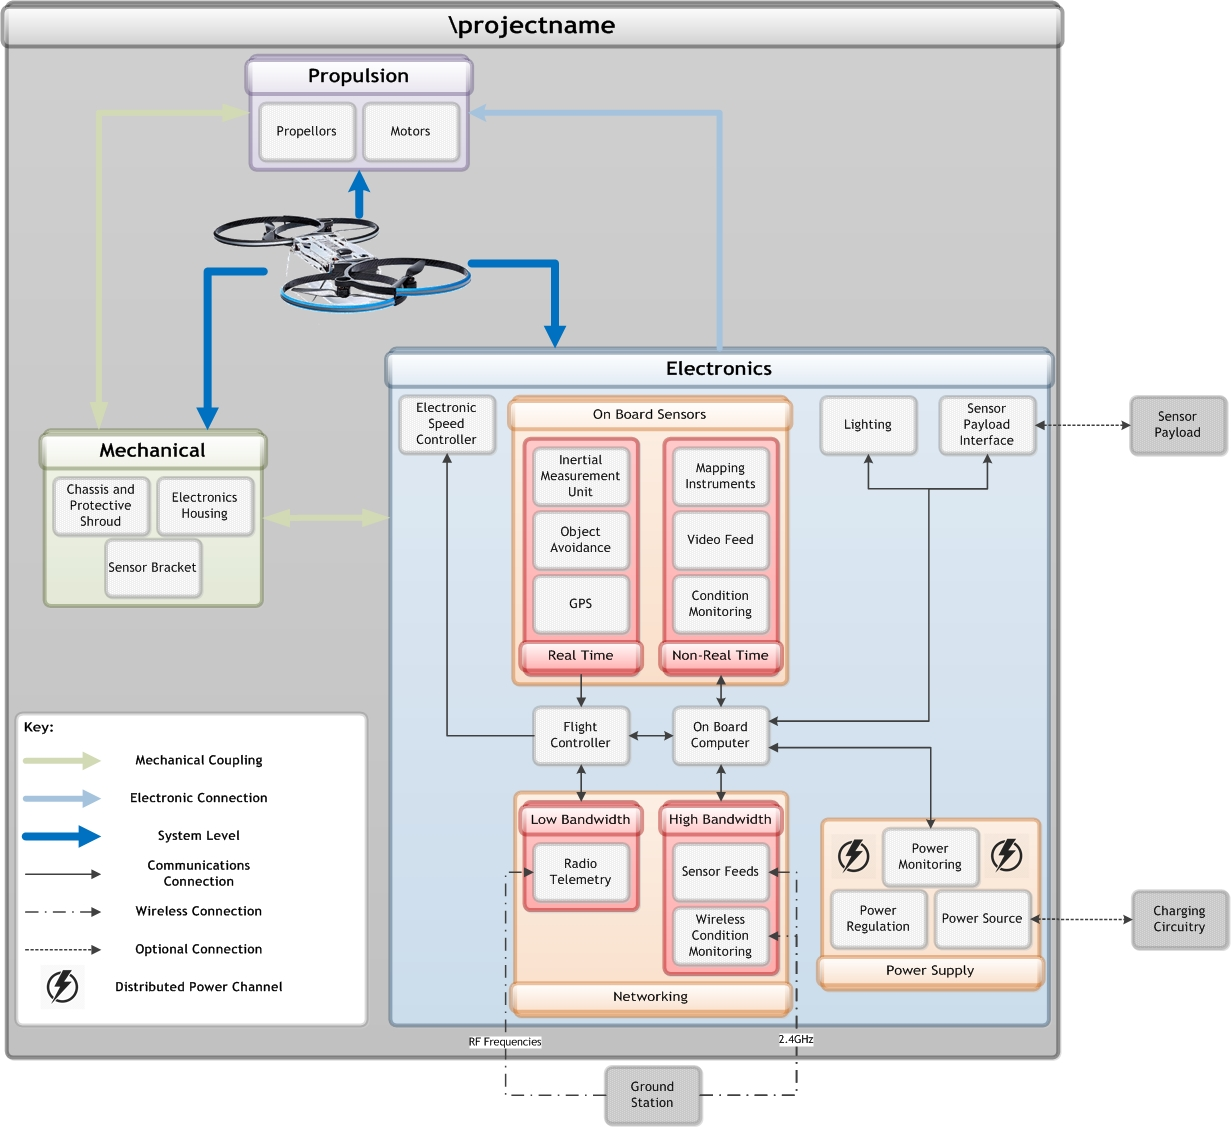
\includegraphics[height = 10cm]{../Design/System/SystemArchitecture/SystemArchitecture.jpg}
		\caption{System Architecture}
		\label{IM_SystemArchitecture}
	\end{figure}
		
		\subsection{Platform Construction}
		The platform is the physical embodiment of the craft. In this context this includes the mechanical construction of the craft, as well as the flight generating components.
		
			\subsubsection{Mechanical Construction}
			The mechanical construction of the system introduces size restrictions for the rest of the system. It should provide adequate mounting for the necessary peripherals described in the sections following. The structure needs to protect the rotors from collisions be means of a shroud and include lightweight landing gear. The chassis must also be such that the weight is distributed as symmetrically as possible. The propulsion system must be housed and provided with rigidity for steady flight control.

			\subsubsection{Propulsion and Flight Characteristics}
			The propulsion system comprises of the motors and propellers. This subsystem needs to supply enough thrust and overhead for steady control, as well as enough lifting capacity to carry any additional, mission sensors. The craft should be able to handle a \payLoadMass payload. To ensure capable disturbance rejection, the total maximum thrust should be no less than $150\%$ of hover.
			
			The craft must efficiently hover and fly at low speeds. The craft should have multiple control surfaces to accurately counter disturbances. Due to the intended use case, the craft will fly with a set orientation and thus does not require the abilities for sharp turns of manoeuvres.
		

		\subsection{Electronics Interface}
		At the core of any reliable robotic platform is a thoroughly planned electronics system, for \projectName this is the most complex subsystem containing the most modules. It is responsible for all intelligence and power generation. This subsection breaks this subsystem into more discrete parts. It begins by separating the two computing modules into real time and non-real time components. The real time components include some of the on board sensors which are required for stable and fast control theories, which all feed into the flight controller. For the drone to successfully navigate an environment it will need to better understand it's surroundings. The flight controller will analyse this data and based on flight software will control the electronic speed controllers. The on board computer will process and handle all non flight critical sensor information and can be considered as the mission computer. The OBC must also have provision to connect to a sensor pack via a predetermined interface. Another useful and necessary function, will be the ability to illuminate a dark area. 
		
		The network design will also consist of 2 discrete wireless links. Each link is dedicated to one of the computing modules. The real time node will be interfaced through a low bandwidth, high range and high reliability interface. With the non-real time node linking to the high bandwidth interface which will have lower range and reliability requirements. Both of these interfaces will link to a ground station of some sort.
		
		No system can operate without a sufficient power source. In the case of any robotic system it is important that every aspect of the design is optimised. To assist with that an electrical analysis is done to help pinpoint some of the major power consuming components. This analysis will also help to evaluate the required power source. The capacity of the power supply is limited by weight and should be optimised to the lifting capacity of the platform. Once the battery chemistry has been decided upon, work can be done to design a robust power management system. Limiting the leakage of every subsystem as well as choosing efficient modules are both part of an effective power management system. To complete the subsystem will require some form of power monitoring as well as an efficient charging scheme.
		
			\subsubsection{Flight Controller}
			The flight controller is responsible for handling all the flight critical sensor data. Using a mixing algorithm it will then output signals to the electronic speed controllers. There are multiple options for flight controllers, all tailored to different applications, platforms and flying styles. Each option has there own level of reconfigurability. For this application it is important that the chosen flight controller allows access to both the inner control loops as well as allows additional sensor data to be added into the architecture. The flight controller is also responsible for handling the pilot commands sent via the radio link, as well as transmitting in flight diagnostic information back to the ground control station.
				
			\subsubsection{Electronic Speed Controller}
			The flight controller will take in information from some of the on board sensors. It then sends a motor control command based on that information to the electronic speed controller (ESC), which directly controls the speed of each motor. This part needs to be chosen based on the maximum amount of current it can handle. At 100\% throttle the current draw of the motor should not exceed 75\% of the ESC's limit. Another important consideration is the ESC's refresh rate and computing speed. The flight controller will be rapidly sending data to the ESC. The quicker the module can respond, the more accurately the platform will fly. 
			
			Each ESC has built in intelligence and will have their own dedicated firmware. Most ESCs will come with built in firmware, which must be tailored for a quadcopter configuration.
			
			\subsubsection{On Board Computer}
			Where the flight controller ensures the craft maintains steady flight, the On Board Computer (OBC) handles all higher level processing. This will include interfacing to the rest of the on board sensors, the sensor pack as well as handling the high bandwidth networking. The OBC should not be required for flight purposes, and can thus be considered as a dedicated mission computer. 
			The OBC should be as light weight as and low power as possible. The OBC must be sufficiently powerful to do real time analysis of camera data. The OBC must have multiple communication ports to easily interface to other sensors.
					
			\subsubsection{Networking}
			This subsystem will handle control commands, flight and diagnostic data or real time sensing information. As described above these have been separated into two distinct categories, low and high bandwidth or alternatively named as high and low range. 
			
				\paragraph{Low Bandwidth, High Range}
				A reliable connection is an important factor to ensure a successful mission the hardware will be validated against it's range, speed, packet loss and ultimately reliability.
						
				The design will incorporate multiple communication peripherals as a fail-safe in case communications are lost to the base station. The pilot needs full control through it and any relevant data that needs to be transmitted will be sent here as well.
						
				\paragraph{High Bandwidth, Low Range}
				The higher bandwidth connection will be used for higher level mission control and data. The high bandwidth link should be able to transmit large streams of data between the craft and the ground control station. 
	
			
			\subsubsection{On Board Sensors}
			
			
			\subsubsection{Sensor Pack}
			The actual sensor pack in question will remain generic. So that the platform can cater for an array of sensing devices and applications. To ensure compatibility, the sensor pack needs to be able to powered as well as communicated to. It will have access to interface directly to the OBC.
	
	
			\subsubsection{Power Supply}
				\subsubsection{Electrical Requirements Analysis}
				\subsubsection{Power Source}
				\subsubsection{Power Regulation}
				\subsubsection{Power Monitoring}
				
	\section{System Software Framework}
	The electronic components gather and collect all the necessary information, the software combines it all and controls the flow of data to obtain stable flight and more. The software system can also be broken down into different operational groups or subsystems. These are, the firmware running the flight controller, the communication protocols used between the software nodes as well as the ground control station. The ground control station although not deployed on the platform, is still mission critical and must be able to display in flight data and send commands to the craft. The last module is the logging and simulation node, which allows for an in depth understanding of untested flight dynamics.
	
		\subsection{Flight Controller Firmware}
		Most commercial flight controllers will come preprogrammed with flight control software. The required firmware blocks are represented in Figure \ref{IM_SoftwareArchitecture} and are discussed in the subsections that follow.
		
		\todo[inline]{Make figure and add in the blocks required}
		\begin{figure}[H]
			\centering
			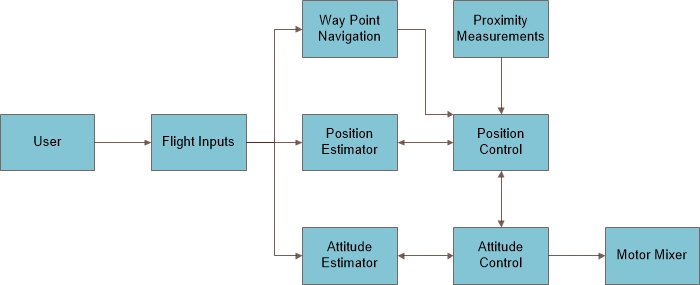
\includegraphics[height = 4cm]{../Design/Software/FirmwareBlocks}
			\caption{Software Framework}
			\label{IM_SoftwareArchitecture}
		\end{figure}
		
			\subsubsection{Flight Modes}
			All the different modules must be accessible and configurable. The flight controller must be able to handle different flight modes that can be changed during a mission. There must be an autonomous flight mode, where the craft can follow set way points. When not in autopilot, the pilot must be able to send the craft commands to control it's movement. 
			
			\subsubsection{Position Controller}
			For precise control, the firmware will need both a well defined position and attitude estimator. 
			The position estimator must accurately predict the current position of the craft and accept new set points based on user defined way points. 
			The position control must create angle and throttle commands to rectify the error calculated in the position estimator. The commands are then sent to the attitude estimator to create new attitude set points. 
			
			\subsubsection{Attitude Controller}
			The attitude estimator must measure the crafts orientation and will be fed information from both the on board positioning monitoring system, as well as the inertial measurement unit. The attitude estimator must be able to take new set points from either the user or the position controller, depending on flight mode. The set points are then fed into the attitude control which calculates the error and generates PWM motor commands that are sent to the ESCs.
			
			\subsubsection{Way Point Navigation}
			As mentioned, the controller must have a way points navigation module, that can feed new position commands into the position estimator. The way points module will need to be able to update during a mission. The way points become the mission goal, to obtain this goal in a confined space, the craft must be able to deviate off course to avoid obstacles. 
			
			\subsubsection{Proximity Sensing}
			Obstacle avoidance calls for a module that can calculate the craft's proximity to it's immediate surroundings. This module will accept information from proximity sensors and output warnings to the position control. The position control must generate a flight strategy that allows for deviations off course, while the total deviation must round to zero.
					
		\subsection{Communication Protocols}
		The communication to and from the craft is represented in \ref{IM_SystemArchitecture}.
			\subsubsection{Radio and Telemetry}
			The radio frequency (RF) must be \todo{insert South African regulation frequency}. This link is a higher range connection and must be able to send commands reliably to the craft. 
			The telemetry link is between the GCS and the craft. It is a higher bandwidth connection and must be able to send in flight data and receive commands from the GCS. More is specified in the ground control software section.
			\subsubsection{Mission Computer}
			\subsubsection{External Sensors}
		\subsection{Ground Control Software}
		The ground station must deploy software that can visualise flight data. The GCS must also be able to send commands to the craft as well as update the mission plan.
			\subsubsection{Data Visualisation}
			\subsubsection{Basic Commands}
			\subsubsection{Way Points}
		\subsection{Logging and Simulation}
		Flight data must be collected and accessible for interpretation and graphing. New strategies can be developed from this data and tested by simulating certain aspects of the hardware.
			\subsubsection{Graphing}
			\subsubsection{Simulation in the Loop}
			\subsubsection{Hardware in the Loop}			
		







					
\chapter{Platform Design}
Obtaining successful flight results with an aerial vehicle will need both precise control algorithms and a robust platform. This chapter contains the technical details of how the final platform decisions was made. The final design will be compared and validated against the proposed outcomes stated above. 

\section{Factors Affecting Design Decisions}
\todo[inline]{not sure about the name of this section}
Before a proper analysis can be done, certain criteria need to be outlined. These include aspects of the project such as the required flight time and manoeuvring decisions. These factors have been drawn up from the proposed research questions and end use case.

\subsection{Physical Restrictions and Requirements}
One of the major components \projectName will have to overcome is to navigate these unknown areas and not only survive collisions, but also reject the disturbances introduced by being close to the walls. Since mine shafts are predominantly long and narrow, the same approach will be looked at for the design of the drone. Hence the platform will be made to be long and narrow. The unique disturbances found in a mine also help define the end configuration as it needs to be able to withstand these disturbances.
Since the drone will be required to navigate very confined spaces, the smaller the drone the better. The minimum size of the drone is limited by the need for adequate flight time as well as payload capacities.

\subsection{Manoeuvring Decisions}
The manoeuvring decisions are dependant on the type of environment and type of missions required by the platform. These decisions influence the final design of the craft.
The end use case for \projectName will include mapping of unknown areas. To complete this, it will simplify the procedure if the drone keeps it's orientation during flight. Due to the nature of the environment, fast speeds will not be used regularly. Therefore \projectName will be designed to have slow, steady and controlled movements. More is discuss in the flight strategy section.

\subsection{Disturbances}
As described above the discussions with CSIR lead to the decision to attempt to use this drone in a mine. Apart from the difficulty of navigating and manoeuvring through an unmapped area there are other disturbances introduced into the system. 
Due to the nature of the tunnels, wind gusts are created that funnel through these passageways. They can reach speeds of up to \todo{Insert Gusts Speed and reference}. Due to the direct relationship between thrust and initial velocity as shown in \eqref{EQ_ThrustMass} any change in wind speed through the rotors will unbalance them.
The effect of coming close to a wall of floor has been discussed in the literature study. The near wall effect will also create an imbalance that creates a moment towards the wall. 
Since the areas will be unknown, collisions and bumps are extremely likely, if not inevitable. The drone must be able to withstand a collision and maintain it's orientation as best as possible.

\subsection{Thrust Overhead}
The total overhead of a rotorcraft is a percentage above the thrust required for hover. This value determines a craft's ability to manoeuvre, with a higher value giving it more freedom and a greater ability to resist disturbances. With these benefits the system does become very sensitive and more difficult to control and stabilise. Since the craft will be in confined narrow passages, the craft does not need to be fast moving. Rather a "slow and steady" pace will be approached. The craft does however need enough power to counteract the disturbances described above. These considerations lead to a value of $150\%$, with $100\%$ being enough thrust to hover. \todo[inline]{Back this up with references from other designs, spoken about later consider removing from here. Maybe reference botom section?}

\subsection{Flight Time}
Flight time is dependant on efficiency/power requirements of the system as well as the capacity of the on-board power source. This is where the designer runs into a catch 22. By adding a larger power source the weight is increased and therefore the platform requires more power to keep itself aloft. Weight is a determining factor for any aerial system and influences flight time, for this reason the weight of every subsystem must be optimised. To ensure the craft can complete a mission it will need a decent flight time. Initial conversations have set 30 minutes as the bottom limit. The original platform might not be able to reach this goal, but once the platform is performing adequately adjustments can be made to the system to optimise weight and power consumption. 

\section{Final Concept Choice}
The traditional configurations of drones are incapable of handling disturbances introduced by being in a confined space and will continue to struggled to overcome this problem\todo{Maybe a bit harsh, but need to validate why we're not using a standard design}. For this reason a few unique designs were considered and a lot subsequently rejected. Although some rejected ideas did help define the final configuration.

\subsection{Rejected Designs}
\subsubsection{Gimball}
The Gimball design as shown in Figure \ref{IM_Gimball} has been discussed thoroughly in the literature. It is definitely the most sophisticated close quarter drone in the world today. It's rolling cage and gimbal design reduces collisions to hardly effect the drone's flight paths at all. Unfortunately it's Co-axial rotors limit the payload capabilities and reduce efficiency of the craft which inhibits the total flight time. The rolling cage also prohibits successful mapping as the orientation of the craft is constantly changing and any sensors inside the cage will be obscured by the rolling protection.

\begin{figure}[H]
\centering
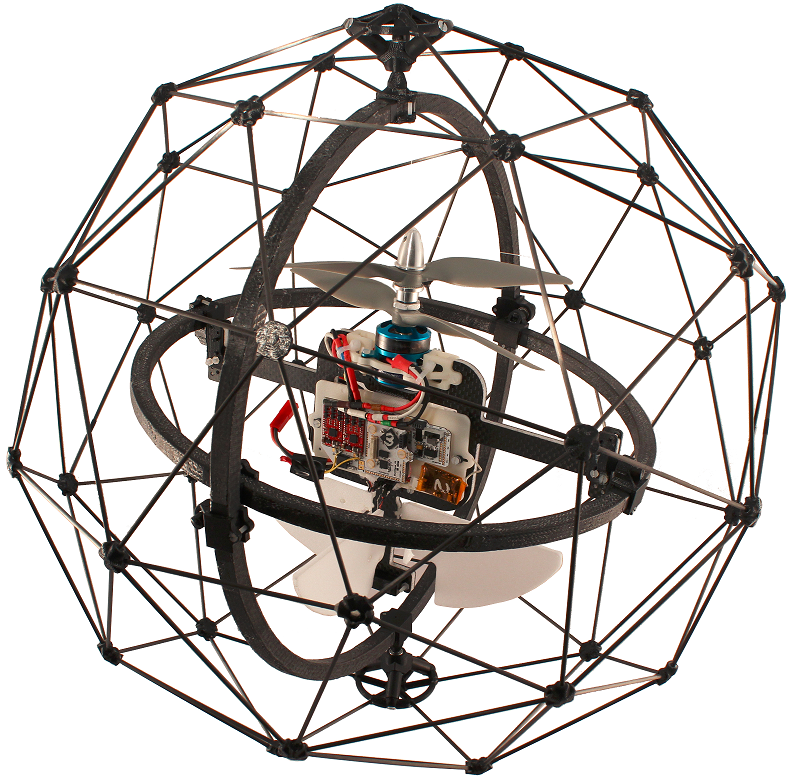
\includegraphics[height = 6cm]{Images/Design/Gimball}
\caption{Flyability's Gimball (Picture taken from http://www.flyability.com/product/)}
\label{IM_Gimball}
\end{figure}

The Gimball is a great tool and will aid a lot of industries, but it was not seen as a viable method to conduct mapping or carry any sort of payload for an extended period of time.

\subsubsection{Tandem Tilt Rotors}
After much thought into the problem a unique design was considered. Figure \ref{IM_TiltTandem} is the initial realisation of that concept. The idea was to capitalize on a tandem's narrow design while giving it more freedom by allowing the rotors to tilt. After the concept had been drawn up it was noted that adding tilt abilities to standard configuration has been looked at and used successfully before \cite{TandemTiltRotor, TripleTiltRotor}.

\begin{figure}[H]
\centering
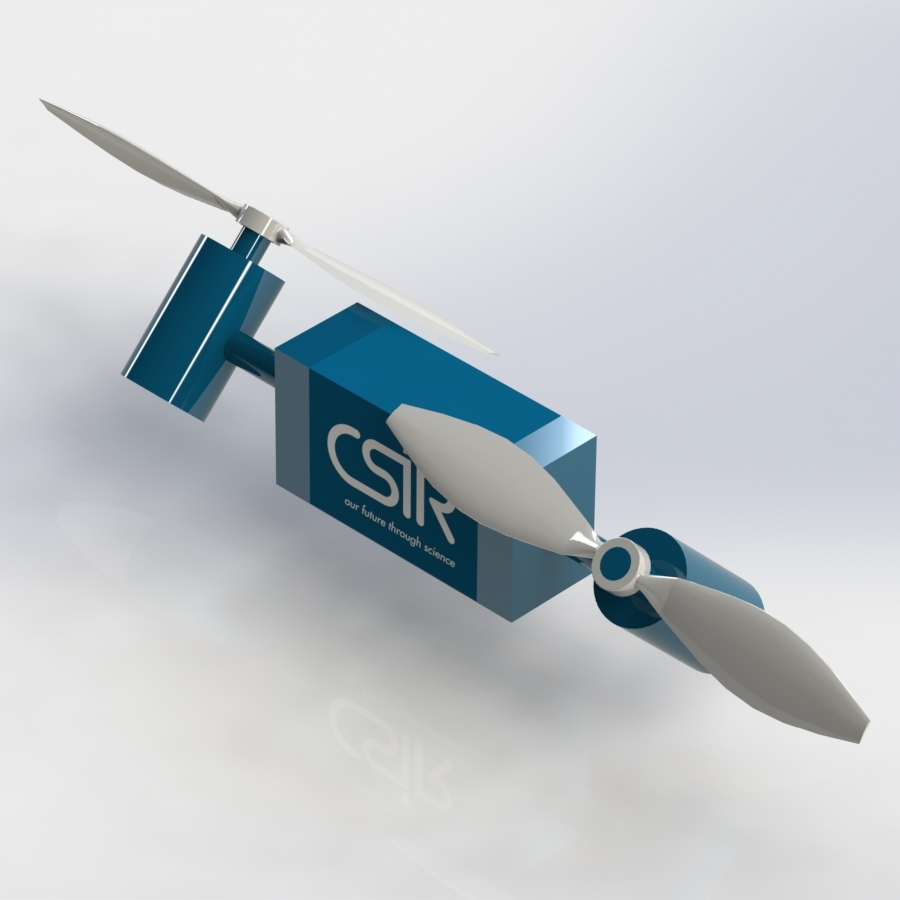
\includegraphics[height = 6cm]{Images/Design/Tandem}
\caption{Rendering of initial concept of the Tandem Tilt rotor Rotorcraft}
\label{IM_TiltTandem}
\end{figure}

The big issue with this design would be controlling the platform. Designing a tilt rotor without variable tilt rotors would not produce enough roll control. The tilt mechanism will help with this, but affect too many other efficiencies while doing it. The tandem will also be more susceptible to disturbances than a four rotor approach.

\subsection{Chosen Concepts}
\todo[inline]{For the comparison, figures were obtained while the following was assumed: Thrust to RPM linear. RPM to current linear. Make sure they are correct}

After much thought two concepts were selected as final candidates. This next section walks through some of the important factors considered and ultimately, why certain decisions were made. 
On the left of Figure \ref{IM_UnlikeSizes} represents the \textit{"Unlike Size Quad"} and the right of Figure \ref{IM_UnlikeSizes} is the \textit{"Overlapping Quad"}. 

\begin{figure}[H]
\centering
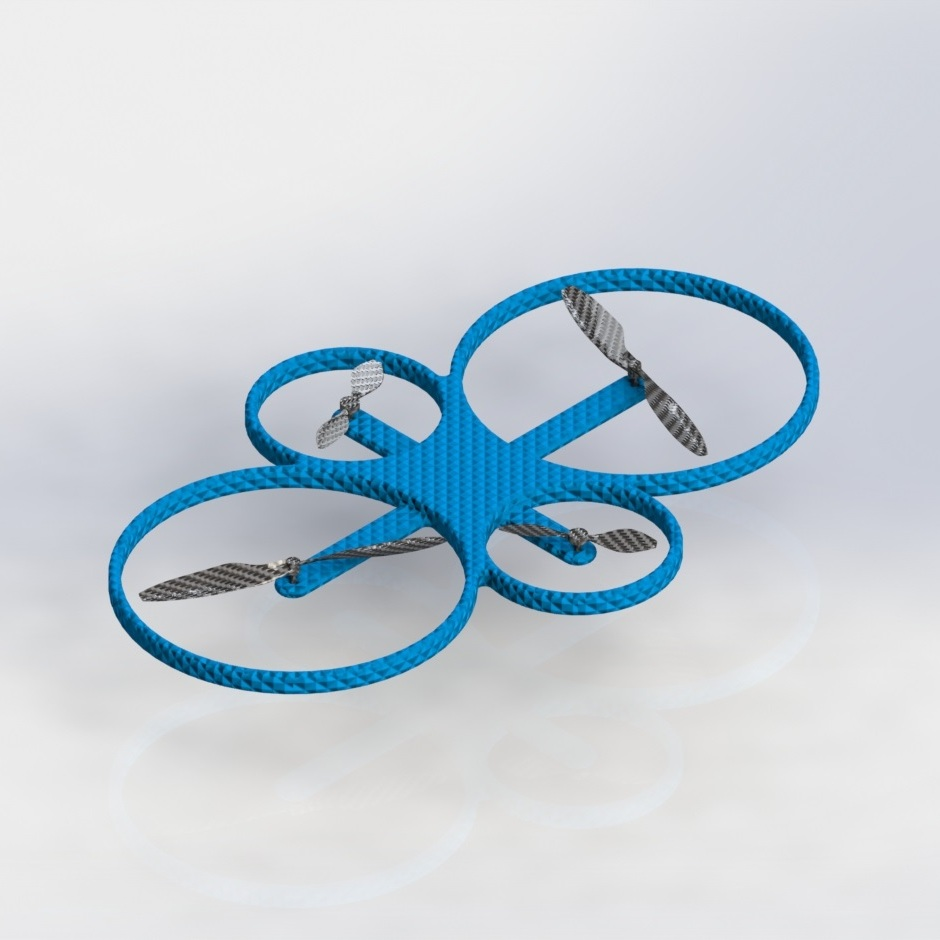
\includegraphics[height = 6cm]{Images/Design/UnlikeSizes}
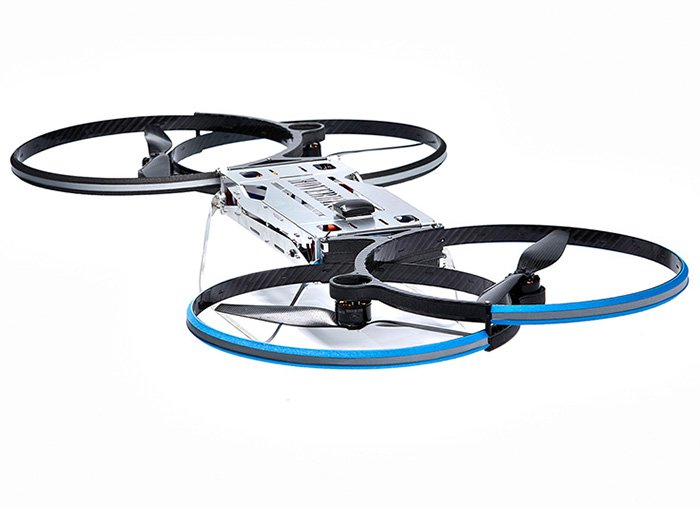
\includegraphics[height = 6cm]{Images/Design/Overlapping}
\caption{a)Rendering of initial concept of the unlike rotor size quadcopter and b) Malloy Aeronautics Hoverbike Concept (Picture taken \cite{MAHover}).}
\label{IM_UnlikeSizes}
\end{figure}


\subsubsection{Concept 1 - The Overlapping Quad}
The overlapping quad is a concept pursued by Malloy Aeronautics \cite{MAHover}. They used the design in an initial concept of their hover bike. The design uses an X-formation for it's rotors, except the rotors are brought in to limit the width of the craft to the point that they overlap, as shown in Figure \ref{IM_UnlikeSizes}. Each overlapping pair will have both spin directions, this feature is shown in Figure \ref{IM_OverlappingPair}.

\begin{figure}[H]
\centering
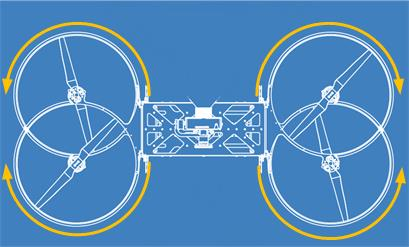
\includegraphics[height = 6cm]{Images/Design/OverlappingVD}
\caption{Overlapping concept, visual representation of rotor pairs. Image modified from \cite{MAHover}}
\label{IM_OverlappingPair}
\end{figure}

If this configuration is selected, there are still other design questions that need to be answered. Overlapping rotors introduce an inefficiency into the system. Johnson in \cite{HeliTheory}, says there is much debate in how the efficiency is calculated. He states two of his preferred methods, the method chosen has a better approximation for small overlaps and is shown in \eqref{EQ_OverlapEfficiency} \cite{HeliTheory}. $\Delta P$ is the interference power (considered here as a fraction of total power) and $m$ is the overlap fraction and is calculated in \eqref{EQ_Overlap} \cite{HeliTheory}.

\begin{equation}
\label{EQ_OverlapEfficiency}
\frac{\Delta P}{P} = (\frac{2}{2-m})^{1/2} - 1
\end{equation}

\begin{equation}
\label{EQ_Overlap}
m = \frac{2}{\pi} \Bigg[ \cos^{-1}\frac{l}{2R} - \dfrac{l}{2R}\sqrt{1 - {\dfrac{l}{2R}}^2} \Bigg]
\end{equation}

These quantities assume a small vertical separation so that the inflow rates of both rotors can be considered the same. To calculate the overlap function, the rotor radius $R$ is needed as well as the separation distance $l$. Figure \ref{IM_SeperationGraph}, illustrates how the separation affects both the  overlap function as well as the total power as a percentage.


\begin{figure}[]
\centering
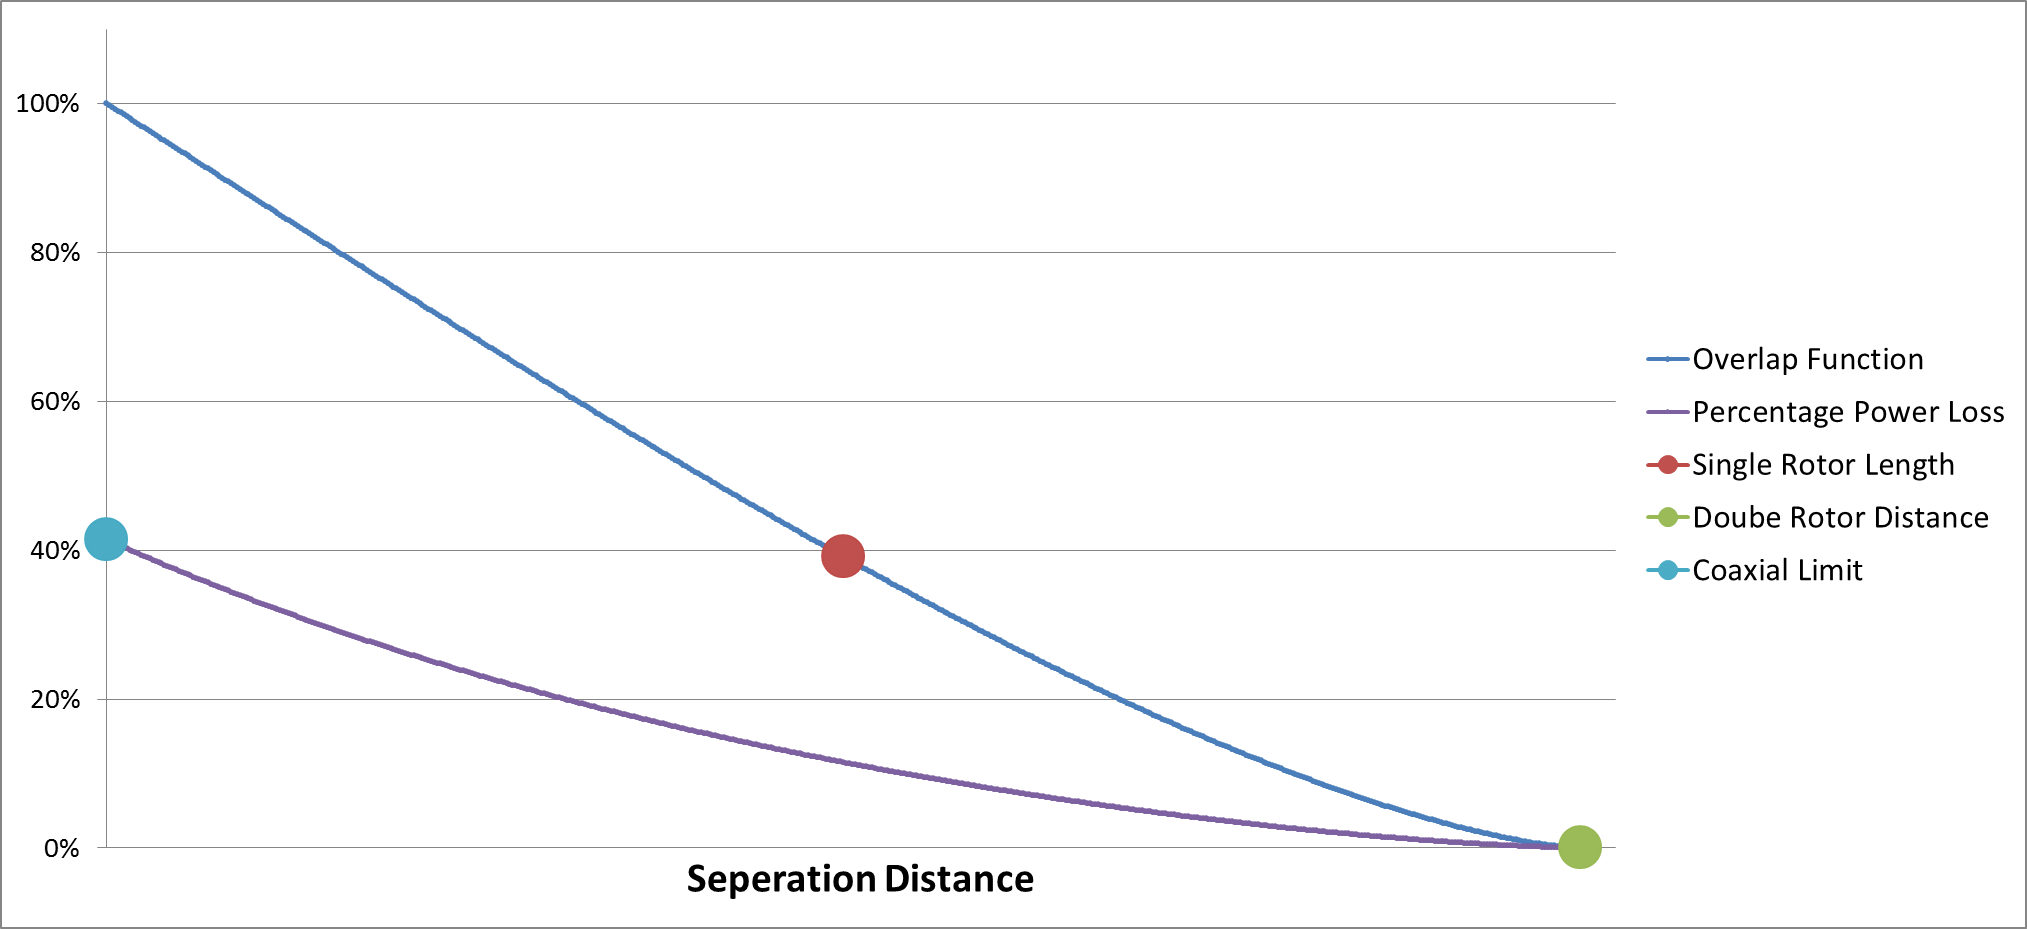
\includegraphics[height = 6cm]{Images/Design/SeperationGraph}
\caption{Graph representing the effects of separation distance in an overlapping quad}
\label{IM_SeperationGraph}
\end{figure}


The length of the craft needs to also be decided, this aspect only becomes critical once payload requirements are factored in. As stated above, this design was an initial concept for a hoverbike with the intended payload capacity of a human. So a big positive to this design is the power to size ratio. This benefit can be utilised through handling larger payloads, or a larger battery pack increasing total flight time.

\subsubsection{Concept 2 - The Unlike Size Quad}
The unlike size quad is an original design that uses the standard cross formation, except it has two pairs of different size rotors. This means that the counter rotating pairs will be set up as shown in Figure \ref{IM_UnlikeSizePair}, with each rotation direction having one big and one small rotor. 

To maintain a common DL in the system the thrust requirement will be lower on the smaller blades and larger on the bigger blade. The smaller the side rotors get, the higher the thrust requirements of the larger rotors become, this limits the rotor size ratio. Initial calculations, factoring in thrust overhead, overall size of the craft and minimum thrust allowed to rotors, set the ratio between $65\% - 80\%$.  When approaching the lower bound, the thrust requirement for hover alone leaves very little room for manoeuvring or disturbance rejection. The upper bound reaches a point where the size difference is so negligible the design's narrow intent is lost.

\begin{figure}[H]
\centering
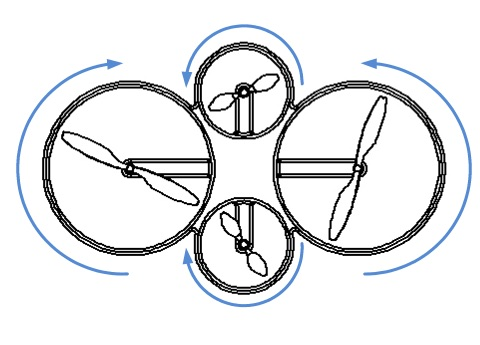
\includegraphics[height = 6cm]{Images/Design/UnlikeSizeRotorPair}
\caption{Unlike Size Quad visual representation of rotor pairs}
\label{IM_UnlikeSizePair}
\end{figure}

The second important choice is how far to put the rotors away from the centre. As the craft gains translational speed, the air doesn't come in directly from the top any more as shown in \ref{IM_MomentumTheoryAirFlow}. Instead it now starts to come in at an angle. As the craft then manoeuvres and changes it's orientation, the air starts coming in at more extreme angles. If the electronics housing has a lot of height it can interfere with the wake boundary and create an inefficiency. This inefficiency is also based on how far the rotors are from the housing. A similar concept is described in Section \ref{SSSECT_NearGroundEffect} Therefore, before this decision can be made the limits of how small the centre electronics housing needs to be decided. 

Through discussions and observations of current systems a minimum limit of $75mm \times 75mm$ was set. To avoid overlap, the distance from the centre of the big rotor and the centre of the craft will be at the very least $R$. Including space for the housing increases this.

The left and right placement is where the originality comes in. Since the craft needs to remain narrow, the side rotors can be brought in as well as shrunk. This would require pushing the two larger rotors slightly more out. Bringing the side rotors in closer to the middle housing will reduce efficiency, so a compromise must be chosen between width and efficiency. Since the side rotors don't contribute as much to the system as their bigger counterparts they have the option of a lower separation distance. The lower separation distance can also be justified by the lower need and use of roll moments and side translations.

Lastly the rotor pitch angle needs to be selected. The major contributing factor of any rotor (besides it's size) is it's pitching angle. As the pitch angle changes, so does the lift to drag ratio. Generally a craft would always want a higher lift to drag ratio, in this case however the side rotors might have a lower lift to drag ratio so they can help counter the torque applied by the larger blades more effectively.

\subsection{Concept Comparison}
After being introduced to the two concepts, they will now be compared based on certain factors. This comparison includes hover efficiency, thrust and electrical power. Lastly size and manoeuvrability are grouped together since they inherently affect each other. The final decision will need to be made with certain assumptions in mind, that must be validated through testing further down the line. These assumptions as well as the method of comparison are described below. 

\subsubsection{Assumptions and Method}
Since both designs use 4 rotors they can be compared relative to a well known design, the standard quadrotor. For each configuration certain parameters need to be decided before a comparison can be done. Using formulas and plots in Microsoft Excel\texttrademark, both designs could be visualised rudimentary as shown in Figure \ref{IM_Excel}.

\begin{figure}[H]
\centering
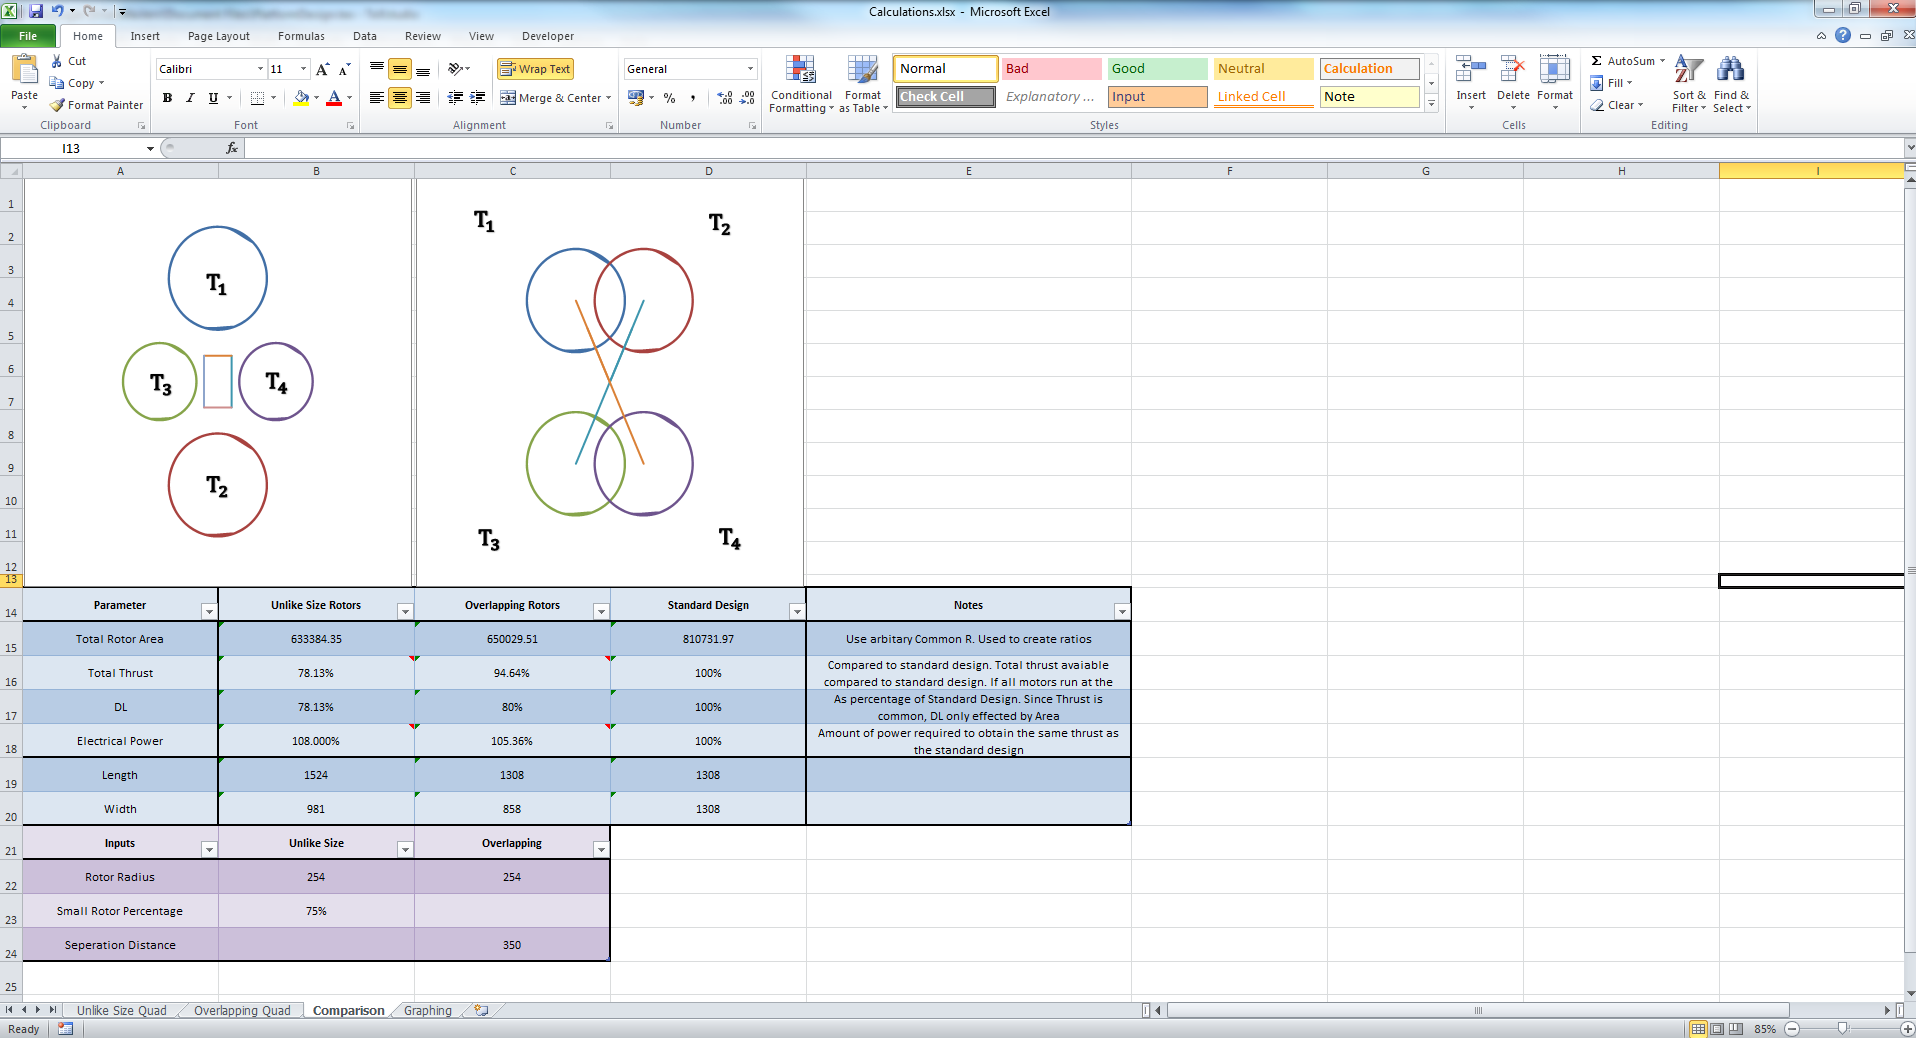
\includegraphics[width = 15cm]{Images/Design/Excel}
\caption{Rudimentary Visualisation of the two concepts using Microsoft Excel\texttrademark}
\label{IM_Excel}
\end{figure}

If hover is a thrust of $100\%$, the overhead was set at $50\%$ \todo{Try and find papers stating other values I want to validate this decision} of that, to a total of $150\%$. Minimum thrust per rotor was set at $20\%$. The mass in question includes provision for a sensor pack of undecided mass. 

The two designs had different decisions that needed to be made. After a bit of trial and error the unlike size quad had it's small rotors set at $75\%$ of the larger ones, this decision is explained further in the text. Just to give a quantifiable reference, R was set at $254mm$. With that assumption the unlike size quad moves it's side rotors in to a distance of $300mm$ and the larger rotors were moved to $508mm = 2R$ away. The overlapping quad set a separation distance of $350mm$ which created an overlap factor of $m = 19.82\%$. 

These values were used to do the following analysis.


\subsubsection{Rotor Area and Disk Loading}
If a rotor size of $R$ is assumed for the rotors\footnote{The big rotors in the case of the unlike size quad} then the total area for a standard quad will be $A_{std} = 4 \pi R^2$. Based on simple geometry, the reduction in radius of the two smaller rotors leads of the unlike size quad leads to a decrease in area. Using $75\%$ this is calculated to $78.13\% of A$. 

As described in \eqref{EQ_Overlap}, the overlapping quad introduces a reduction in total disk area, with an overlap factor of $19.82\%$ leaves a total area of $80.18\%$. Since the thrust requirements are assumed the same, the disk loading ratios will be exactly the same as the area ratios.

\subsubsection{Thrust and Power Considerations}
The $75\%$ decision was based on observation of thrust ratios and comparing them to the minimum and maximum values stipulated earlier. This decision must also be influenced by available rotor sizes and pairings. The final value graphs are shown in Figure \ref{IM_ExcelGraphs}. The thrust percentage per rotor is shown, the points marked are at minimum, hover and maximum. Equation \eqref{EQ_ThrustMass} states that thrust is proportional to area. Therefore the reduction in rotor area will cause a directly related reduction in thrust. The total thrust available to the unlike size quad is $\approx 78\%$ of the thrust available to the standard design. This reduced value also comes at a weight reduction. The overlapping quad has an equal total rotor area but an inefficiency is introduced by the overlap as according to \eqref{EQ_OverlapEfficiency}. Therefore the overlapping quad has $94.64\%$ of the total thrust, without the weight reduction.

\begin{figure}[H]
\centering
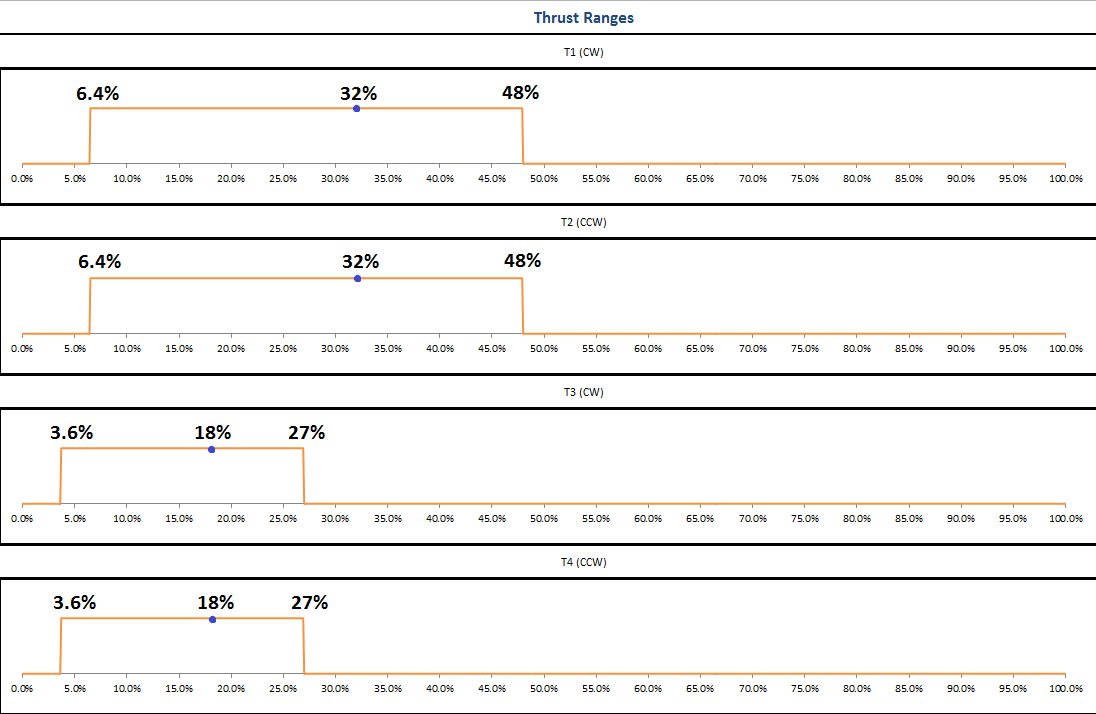
\includegraphics[height = 10cm]{Images/Design/ExcelGraphs}
\caption{Graphical representations of the thrust ratios for the unlike size quad}
\label{IM_ExcelGraphs}
\end{figure}

As for the electrical power, the values were calculated according to how much energy would be needed to obtain the same thrust as the standard design. The inefficiency introduced by the overlap relates to a reduction in thrust of $\Delta T_{overlap} = 5.36\%$, therefore $\Delta P_{overlap} = 14.21\%$ is needed to overcome this loss, based on \eqref{EQ_ElectricalPowerThrust}. 

For the unlike size quad, the reduction in rotor size leads to a substantial loss in aerodynamic power, even with a small reduction in inertia. To regain that power, the rotors need to be pushed harder, this leads to an increase in electrical power. A value of $\Delta P_{unlike size} = 18.5\%$ can be calculated under certain assumptions.

\subsubsection{Size and Manoeuvrability}
The size was calculated as though the drone made a rectangular box and with the rough values above, Table \ref{TAB_SizeComparison} puts those values in a tabular format.

\begin{table}[H]
	\centering
	\begin{tabular}{l | c | c }
		Concept & Length ($mm$) & Breadth ($mm$) \\
		\hline\hline
		Unlike Size	   	& 1524 & 981 \\
		Overlapping    & \boldmath$1308$ & \boldmath$858$ \\
		Standard		& 1524 & 1524\\
	\end{tabular}
	\label{TAB_SizeComparison}
	\caption{Table representing the size comparison of the two concepts}
\end{table}

As shown Both crafts are similar in size, with the overlapping design being slightly shorter as well as more narrow. 

This narrowness comes at a cost. Moments ($M$) are created by a difference in forces($\Delta$) and is multiplied by the distance between the forces ($l$) $M = \Delta Fl $. In the case of the overlapping rotors, the distance between the two different thrust vectors is not as tangible as the unlike size design. This gives the unlike size quad the advantage as bigger moments can be created\todo{Need to make this quantifiable}, allowing for more advanced manoeuvrability and disturbance rejection. However in the case of the near wall effect, the disturbance is created by effecting only one rotor . In the case of the overlapping rotors, the disturbance might be slightly diminished as both rotors will feel the effect. This can be verified later by comparing gathered data to literature. \todo{Would be cool to come back and do this later and reference it here}


\section{Platform Conclusions}

The quantifiable values are culminated below in Table \ref{TAB_ConceptComparison}. The winner of each parameter is written in bold.

\begin{table}[H]
	\centering
	\begin{tabular}{l | c | c | c | c | c }
		Concept & Disk Loading & Total Thrust & Electrical Power & Length ($mm$)& Width ($mm$) \\
		\hline\hline
		Unlike Size	  & \boldmath$78.13\%$  & $78.13\%$ 	& $118.57\%$	& $1524$ & $981$ \\
		Overlapping    & $80.18\%$ & \boldmath$94.64\%$  & \boldmath$114.21\%$	& \boldmath$1308$ & \boldmath$858$ \\
		\hline\hline
		Standard		& $100\%$ 	& $100\%$  	  & $100\%$			& $1524$ & $1524$\\
	\end{tabular}
	\label{TAB_ConceptComparison}
	\caption{Table representing the end comparison of the two concepts}
\end{table}

Now to make the final decision all the factors need to be included. What is known now is that the overlapping quadrotor is superior in almost every quantifiable way. The manoeuvrability aspect is not critical to this application as the use case will involve extremely steady flight. The disturbance rejection of both crafts will be good with 4 rotors. 

Malloy Aeronautics sell what is called a \textit{Drone-3 Kit}, it includes various accessories to help developers use the platform. The novelty of the unlike size rotor quad can now be seen as a negative since it requires a custom frame and shroud.

Based on the above analysis and conclusions the overlapping quadrotor design will be used as the design going forward.

\section{Drone 3}
\subsection{Assembly}




\chapter{Electronic Design}

At the core of any reliable system is a thoroughly planned electronics system. There are multiple aspects this subsystem must handle. Due to the rapidly increasing market and interest in multirotors there has been a wave of developers and designers creating devices for these specific purposes. The first and foremost is monitoring and controlling flight dynamics. This requires flight, speed and motor controllers.	

The on board computer will handle the data streams and control the non-real time peripherals. The device also needs to have networking capabilities to allow wireless communication during flights. For the drone to successfully navigate an environment it will need to better understand it's surroundings. To achieve successful navigation, a few onboard sensors have been looked at. Another useful and necessary function, will be the ability to illuminate a dark area. This will allow surveillance and condition monitoring of these unlit zones. Another design consideration is the provision for a sensor pack. This section of the study involves looking at potential external sensors and providing accessibility for them.

No system can operate without a sufficient power source. In the case of any robotic system it is important that every aspect of the design is optimised. To assist with that an electrical analysis is done to help pinpoint some of the major power consuming components. This analysis will also help to evaluate the required power source. The capacity of the power supply is limited by weight and should be optimised to the lifting capacity of the platform. Once the battery chemistry has been decided upon, work can be done to design a robust power management system. Limiting the leakage of every subsystem as well as choosing efficient modules are both part of an effective power management system. To complete the subsystem will require some form of power monitoring as well as an efficient charging scheme. Since every aspect of the design must consider weight, the charging plan will inevitably involve an external charging device.
		
		\section{Flight Controller}
		If the	OBC is the brain of the system, the flight controller is the nervous system\todo{think of a better analogy}. There are multiple options for flight controllers, all tailored to different applications and flying styles.
			
			\subsection{Custom Design}
			Given the time and resources most final products will look at custom designing some hardware and electronics. The benefits of custom design include complete control over the operation and functionality of the design as well as reduced cost when scaling up. The development of a custom design however can be very taxing and costly.
		
			It is also common for a research lab to dedicate time into developing such modules. By using MITs custom board, Cutler in his masters dissertation demonstrates this \cite{How2012}. \textit{The University of Stellenbosch's Electronics System Lab} produced a custom design in \todo{insert date the boards were designed and reason we're not using them}. This board is under redesign and unfortunately cannot be used for this project.
			
			\subsection{Pixhawk}
			The need for a commercial solution becomes evident. Due to the growing hobbyist community, some flight controllers are difficult to modify and are designed for use as a \textit{"plug and play"} module. Fortunately there is also a large designer community which has created the need for more configurable modules.
			
			 Figure \ref{IM_Pixhawk} shows the \textit{Pixhawk}, which is marketed as an autopilot module for fixed and rotor craft as well as boats and even cars. It is specifically tailored for research and is listed as open-hardware\footnote{https://store.3dr.com/products/3dr-pixhawk}. Due to the open platform it has created an experienced community with many wiki pages and other forms of assistance.
			
			\begin{figure}[H]
				\centering
				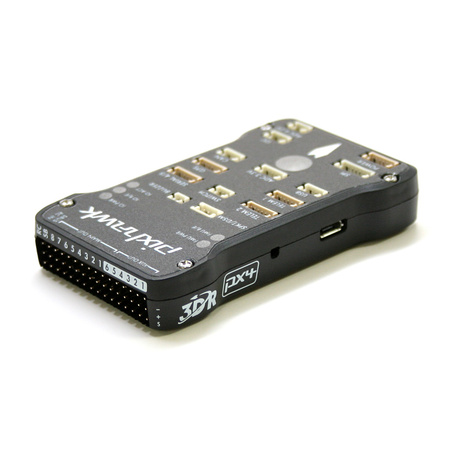
\includegraphics[height = 6cm]{Images/System/Pixhawk.jpg}     
				\caption{Pixhawk Flight Controller}
				\label{IM_Pixhawk}
			\end{figure}
			
			It features a 32 bit STM32F427 processor, running at 168MHz with 256Kb of RAM and a 2Mb Flash. It comes equipped with a full inertial measurement unit (IMU), consisting of a gyroscope, accelerometer and magnetometer. There is also an integrated barometer to adjust flight patterns as the air pressure fluctuates. It has an additional 32 bit co-processor that acts as a failsafe. It has multiple interfacing capabilities as well as a built in power protection unit\footnote{https://pixhawk.org/modules/pixhawk}. 
			
			The Pixhawk has been designed for robotic applications thus is light weight and power efficient. It operates on a real time operating system called \textit{NuttX} which has Unix characteristics but is much lighter than a different operating system such as Linux. This provides a lot of reconfigurability which is wanted in this project.


		\section{Electronic Speed Controller}
		The flight controller will take in information from the onboard sensors. It then sends a motor control command based on that information to the electronic speed controller (ESC), which directly controls the speed of each motor. This subsystem needs to be chosen based on the maximum amount of current it can handle. At 100\% throttle the current draw of the motor should not exceed 75\% of the ESC's limit. Another important consideration is the ESC's refresh rate and computing speed. The flight controller will be rapidly sending data to the ESC. The quicker the module can respond, the more accurately the platform will fly. 
		
		Each ESC has built in intelligence and will have their own dedicated firmware. Most ESCs will come with built in firmware, the design must be tailored for a quadcopter configuration. If not most common ESCs can be reflashed with downloadable open-source software\footnote{http://www.rcgroups.com/forums/showthread.php?t=1513678}.
		
			\subsection{Drone 3's ESC}
		
		\section{On Board Computer}
		Where the flight controller ensures the craft maintains steady flight, the On Board Computer (OBC) handles all higher level processing. This will include interfacing to the on board sensors, the sensor pack as well as handling most of the networking. In an aerial application weight and power consumption are both important considerations. The OBC will have to process streams of data at fast rates to successfully navigate the drone. Based on current available commercial products a few were selected. The advantages and disadvantages of each will are described below.
			
			\subsection{Raspberry Pi 3 Model B}
			
			The Raspberry Pi has become a well known and respected piece of hardware. It has generated a large community and thus resources are readily available and the device can be bought locally. The new version of the device runs a 1.2GHz 64-bit quad-core ARMv8 CPU and includes built in Bluetooth and WiFi modules, an image from the Raspberyy Pi website is shown in Figure \ref{IM_Pi}\footnote{https://www.raspberrypi.org/products/raspberry-pi-3-model-b/}. 
			
			\begin{figure}[H]
				\centering
				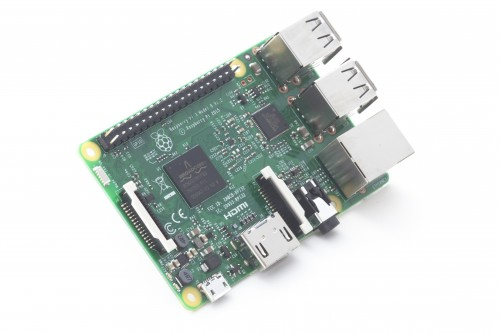
\includegraphics[height = 6cm]{Images/System/Pi.jpg}     
				\caption{Raspberry Pi 3 Model B}
				\label{IM_Pi}
			\end{figure}
						
			It has a large 40 pin GPIO connector, 4 USB connections and an Ethernet port. The Pi's main advantage would be the access to the online community constantly updating Raspberry Pi wikis and forums. With the community also comes example projects and large variety of compatible hardware and open source software. With a maximum current of 2.5A at 5V, the 12.5W computer is relatively low powered which suits this application. However there are more powerful machines that can run more intense algorithms at the cost of more power.
			
			\subsection{Odroid XU4}
			A Korean company, Hardkernel has designed a compact high processing power unit called the Odroid XU4. It has gained respect in some developer communities due to it's incredible processing power. It can run both Android, Ubuntu and other similar Linux based operating systems. Hardkernel has generated an immense of documentation and wiki pages, all available on their website\footnote{http://www.hardkernel.com/}. They also have a team of developers creating new devices to interface with the devices. 
			
			\begin{figure}[H]
				\centering
				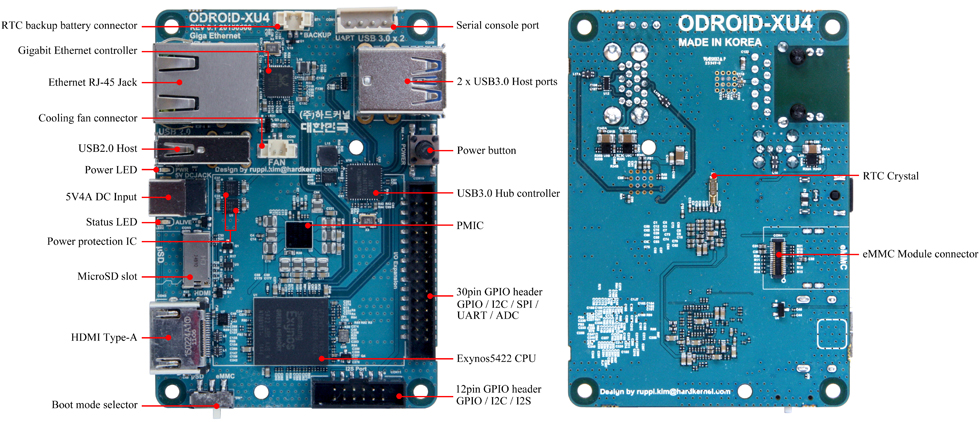
\includegraphics[height = 6cm]{Images/System/XU4.jpg}     
				\caption{The Odroid XU4}
				\label{IM_Odroid}
			\end{figure}
			
			The XU4 hosts a formidable Samsung Exynos5422 Cortex™-A15 processor running at a 2GHz clock speed and an additional Cortex™-A7 Octa core processing unit. This allows for incredible processing capabilities and speed, an image from Hardkernel's Website is shown in Figure \ref{IM_Odroid}. The rated power supply for the unit is a 4A at 5V module. Including a 20W module on board will add a significant drain on the power source. It comes with 2 stable USB 3.0 ports and an additional USB 2.0 connection. 
			
			The Odroid is also frequently used at the CSIR, opening up experience and knowledge on the devices.
			
		\section{Networking}
		A robot that is required to navigate areas where humans cannot access requires a wireless networking solution to send and receive data. This data could be control commands, flight and diagnostic data or sensing information. A reliable connection is an important factor to ensure a successful mission and will be validated against it's speed, packet loss and ultimately reliability.
		
		Generally applications that require far distance use radio frequencies as their means of communication. There are other options, some of which are explored and compared in a design of an intelligent street light \cite{StreetLight}. Here Leccese looks at Bluetooth, WiFi and compares them to a ZigBee module, although the application is different the review of the wireless networking can be useful. 
		
		The ZigBee module is a more useful platform when creating a network containing many devices that all need to interconnect. It has incredible low power abilities and could be looked at further down the line for creating a wireless mesh network in an underground mine to better communications. Bluetooth has limited range and doesn't produce adequate performance for this application. WiFi could also be a good communication system and can be looked at for point to point communication to the OBC. WiFi has decent range with high transmission speeds creating a more power hungry system compared to the ZigBee modules and other RF devices.
		
		The design may also look at including multiple communication peripherals as a fail-safe in case communications is lost to the base station. The base station will be the control point for the craft. The pilot needs full control through it and any relevant data that needs to be transmitted will be sent here as well.
		
		

		
		\section{Location}
		An important part of any robotic application is localisation. As stated earlier, an underground environment limits the use of traditional GPS. Stellenbosch University as well as the CSIR are both funding research into localisation in a GPS constraint environment \todo{Would be great to cite Natasha or ESL here}. Until such a time that these technologies are readily available, this project will work with traditional GPS devices.
			
		As discussed previously, this project will not be designing for a GPS constraint environment. Fortunately there are many commercial  GPS modules available for purchase. Each with their own advantages and disadvantages. For this project the module needs to be lightweight and low power. The GPS needs to create speed and translation data, this information is crucial when generating maps of unknown areas. The PixHawk website recommends the 3DR uBlox GPS kit\footnote{https://store.3dr.com/products/3dr-gps-ublox-with-compass}. Although many alternatives exist, the open source hardware status creates ease of integration and support. With these considerations, this module has been chosen.
			
		It weighs a total of 16.8gs and as has a low 8.5mm profile. With an update rate of 5Hz and built in compass. This module will perform adequately and fulfil the design needs of the project.
			 
		\section{Object Avoidance}
		Due to the mature of the project object avoidance is deemed an important attribute to design for. This requires that the drone has an understanding of it's environment. This information can then be used in higher processing nodes to actively avoid objects. A few different sensor variations are observed below. 
	
			\subsection{Time of Flight}		
			The first and most common would be using a time of flight (TOF) sensor, such as an ultrasonic transducer. Very similar to bats, a sonar module will emit a pulse and based on the time it takes for the signal to return the distance can accurately be measured. A sonar is dependant on a lot of variables and would require calibration for the environment it is in. Due to the method the modules acquire information the drone will be receive a speed limitation, this fortunately agrees with the desired steady flight dynamics. Since the sonar is dependant on the density of the medium it travels through, disturbance created by the rotors could severely affect the performance of the sensors.
			
			Another option in the same category would be to use an infra red (IR) transceiver in the same configuration. The system uses strobed IR pulses to monitor the distance of an object, the system depends on the ratio of reflection for the IR spectrum. If an object as a high refraction ir absorption ratio the signal can get lost. Ambient light can also cause interference, although most modules will have built in filters.
			
			Using the same base technology TOF cameras have been developed such as Microsoft's Kinect. Instead of a single point, a TOF camera projects an IR grid into the area it wishes to explore. By measuring deviations in the expected grid structure, distance information can be inferred. In an IR rich environment, TOF cameras can get overwhelmed and produce unreliable results. Due to the projection, the power requirements of such a system can also be high.
			
			\subsection{Image Processing}
			The term image processing has been used here to discuss a system that can extract data through a camera feed. It is well known that stereo vision can produce 3D information from multiple 2D images. Although more processing is required, very good results can be obtained form this set up. Generally these systems can be slow and clunky with a high power draw and weight due to the multiple required modules. Using multiple camera streams can also be a relatively slow process, thus limiting the speed of the craft severely.
		
			However, reliability from a robust image processing unit will be more reliable and consistent than a different system. Barry in his PhD developed such a design that minimises the discussed negative effects \cite{Barry2016}. Using this design MIT could obtain object avoidance at speeds of 31mph, proving the effectiveness of the object avoidance system.
			
			Regardless of the modules chosen, object detection and avoidance will be looked at in more detail further into the project.
			
		\section{Lighting}
		Since the drone is required to conduct surveys of unknown areas, the possibility exists where the platform is required to illuminate the area it needs to monitor. This requirement hints at the need for an embedded lighting system. Bright lights can be a power hungry system even if designed correctly. The exact specifications will be discussed further in the text but does not form part of project scope.
		
		LEDs will be used for their performance, longevity and power saving characteristics. They will require an LED driver with dimming capabilities to limit the power usage when full brightness is not needed. The illumination will be able to help the sensor pack gather credible surveying data
		
		
		\section{Sensor Pack}
		The actual sensor pack in question is remaining generic. So that the platform can cater for an array of sensing devices and applications. To ensure compatibility, the sensor pack needs to be able to powered as well as communicated to. It will have access to interface directly to the OBC.
		
		The actual sensing element could vary between 
		\todo[inline]{Lidar}

		\section{Power Supply}
			\subsection{Electrical Requirements Analysis}
			\subsection{Power Source}
			\subsection{Power Management}
			\todo{Power Monitoring}
			\todo{Charging Scheme}



\chapter{Software Design}

	\begin{figure}[H]
		\centering
		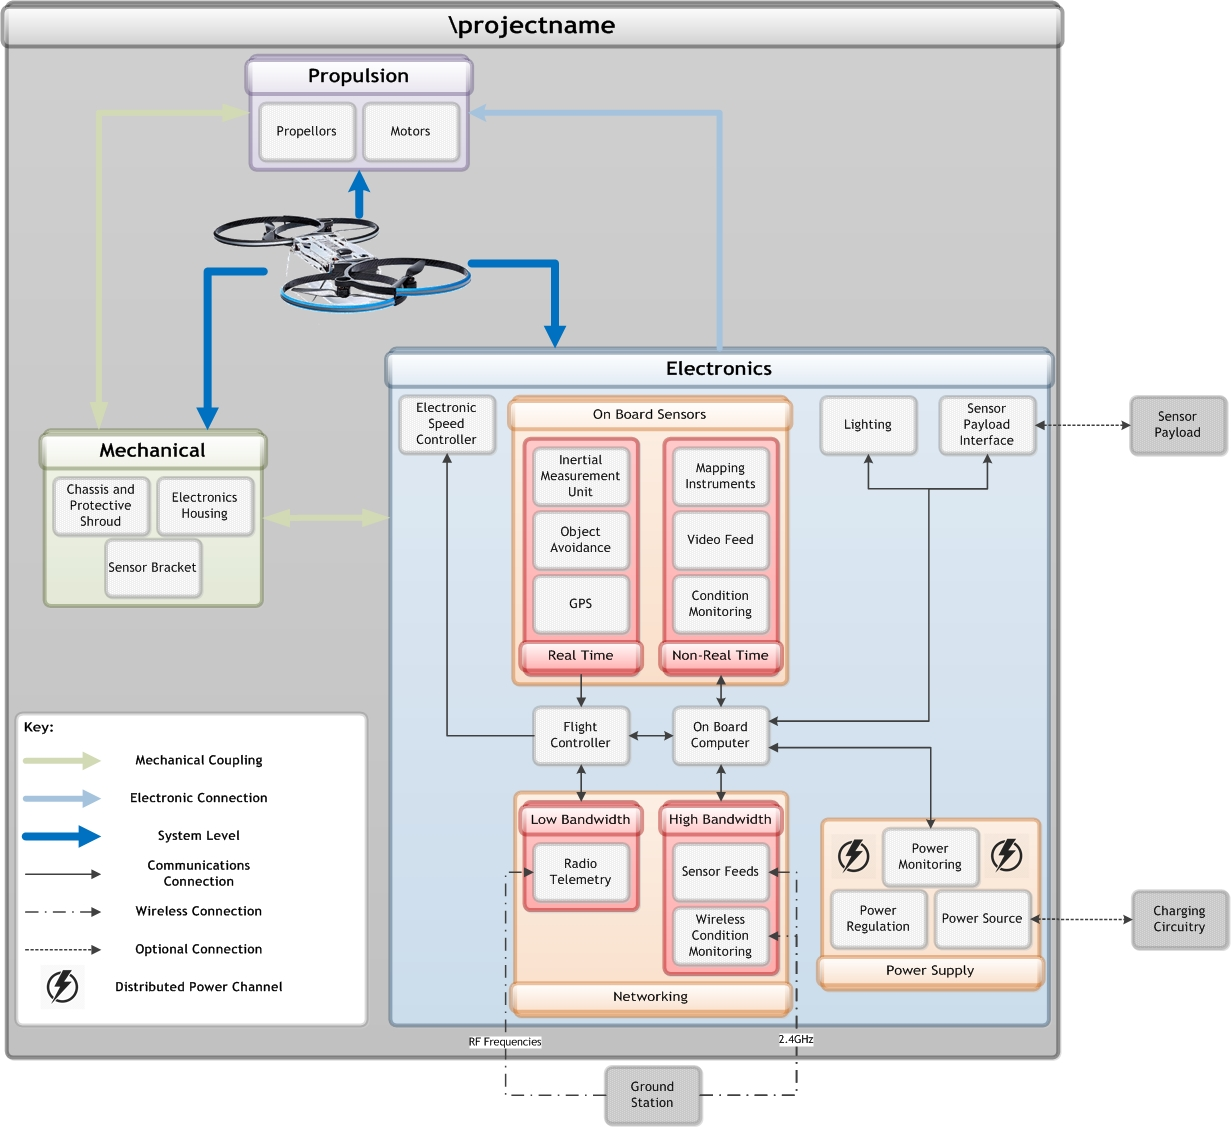
\includegraphics[height = 10cm]{../Design/System/SystemArchitecture/SystemArchitecture.jpg}
		\caption{Software Framework}
		\label{IM_SoftwareArchitectureExpanded}
	\end{figure}


	\section{Flight Strategy}

%\chapter{Removed}
\section{First}
\subsection{Operational Environment}
\todo[inline]{Need to decide if I should keep this in} 
Operating devices in hazardous environments are at times necessary and unavoidable. In the context of this paper a hazardous area is defined as an environment where there is a risk of fire or explosions due to the presence of sufficient quantities of flammable liquids, gases and dusts present in the atmosphere \cite{RockwellAutomation, STAHL}. There are two sets of area classifications, the International Electrotechnical Commission System for Certification to Standards  Relating to Equipment for Use in Explosive Atmospheres (IECEx) which was developed by North America. The European system gets it's name from a French term "Atmosph\`{e}res Explosives" and shall be dubbed ATEX \cite{ATEX, RockwellAutomation, STAHL}.

\subsubsection{IECEx Classification}
The IECEx system breaks up hazardous environments into different classes and divisions which are pertinent to the design of devices to be used in these regions. The varying definitions come with a set of different procedures and regulations that need to be adhered to. The North American classification system, has been designed to give a description of the possible quantities and type of volatile elements in the system \cite{RockwellAutomation, IECEx}.
 
\paragraph{Class Definition}
Three classes are defined and relate to the types of hazardous materials found in the environment. A Class 1 location is an area where flammable vapours and gases are present. Class 2 locations refer to the presence of flammable dusts, such as a coal mine. Finally a Class 3 location is defined as an area containing flammable fibres \cite{RockwellAutomation, IECEx}. 

\paragraph{Division Definition}
The division separation refers to the possibility of the substances, defined in the classes, to be present. Division 1 is defined as an area where the hazardous material will be present frequently. Division 2 states that during traditional operations there is less chance of the substance being found but  may become present through a fault \cite{RockwellAutomation}. 

The IECEx system further breaks down the classifications into groups but for the purpose of this paper it will be assumed that the device must operate in the most flammable gases.


\subsubsection{ATEX Classification}
Where the IECEx system breaks up the different areas into classes and then divisions, the ATEX system simply breaks them up into zones. These zones encompass the full detail of the frequency and the type of hazardous substances.

\paragraph{Zone Definitions}
There are six different zones, the first three zones all relate to the presence of a flammable gas or vapour. Zone 0 defines a gaseous atmosphere which is present continuously or for long periods. Zone 1 is an area where a dangerous cloud is likely to form during operations and Zone 2 is where an explosive atmosphere is not likely to occur and if it does will only be present for a short period of time. Zones 20, 21 and 22 are the designators for dust particles and have the same progression of frequency \cite{ATEX, SANS}.

\subsection{Gas and Temperature Groups}
Both the ATEX and the IECEx classification systems can be further broken down into different gas groups as well as temperature classes. The gas groups are defined by the explosive properties of the materials and are shown in the table below.

The temperature classes are determined according to the maximum allowable surface temperature before an ignition is caused. Both classification systems use the same limits to separate the classes, the difference being that the American system breaks up the classes into sub-classes for more specific definitions.
The ATEX systems varies from a maximum allowable temperature of 450\textdegree (Class T1) to a maximum allowable temperature of 85\textdegree (Class T6) \cite{ATEX, STAHL, SANS}.

\begin{table}[!]
\centering
\begin{tabular}{l | c | c}

Gas Element & IECEx Group & ATEX Group\\
\hline\hline
Acetylene & A & II C\\
Hydrogen & B & II C\\
Ethylene & C & II B\\
Propane & D &  II A\\

\end{tabular}

\caption{Gas groups according to classification systems}
\end{table}

\paragraph{Equipment Categories}
The ATEX definitions also include corresponding equipment categories. Once the device is certified under a specific category, it can be utilised in that category's prescribed zones. Category 1 equipment is considered the most protected and safe devices, they may operate in Zone 0 and Zone 20 and all lower rated zones. Category 2 is the second most rigid equipment group and can be utilised in Zone 1 and Zone 21, as well as the lower zones. Category 3  equipment may only be used in Zone 2 and Zone 22 \cite{ATEX, SANS}.



\subsubsection{Effects of Abnormal Atmospheric Conditions}
Due to the environment in the above mentioned hazardous areas containing mixtures of gases, some atmospheric properties differ from regular air. These conditions could affect the technical operations of certain devices \cite{HC} and for aerial vehicles it is extremely important that the designer has an understanding of the environment the rotors will be flying in \cite{Leishman}. 



%RESEARCH INTO INTRISIC SAFETY
\subsection{Designing for Hazardous Locations}
When designing for hazardous and volatile environments there are stringent standards that need to be followed. The classifications described above determine the level of protection needed in the devices. The main cause of concern in these areas is the generation of fire or equivalent ignition sources, which could cause an explosion.
There are numerous amounts of methods to design in volatile environments. Each of which comes with a set of standards defined by The International Organisation of Standards (ISO). In South Africa the set of standards used are created by the South African Bureau of Standards (SABS) and is documented in a South African National Standards (SANS) document.

\subsubsection{Explosions}
\cite{RockwellAutomation, STAHL}
\paragraph{Causes}
\paragraph{Control}

\subsubsection{Flame/Explosion Proof Enclosures}
A flame proof enclosure is defined by the South African National Standards (SANS) as an enclosure that contains parts which could cause an ignition. The casing must be able to withstand the pressure created by an explosion and not allow the energy to escape and create a further reaction with the explosive atmosphere \cite{FProof}. Each door or cover into the enclosure needs to be accessible only through the manipulation of a threaded fastener. 

\paragraph{Interconnecting Joints}
Spigot Joints
Serrated Joints
Threaded Joints 
Gaskets, O Rings and seals

\paragraph{Operating/Rotating Shafts}
Provision for wear and tear (Gap enlargement)
Cylindrical Joint, labyrinth joint
Gap Diagram

\paragraph{Bearings}
at least one element must be non sparking
Sleeve bearing not permitted for $\mathrm{II}$C
Rolling-element


\subsubsection{Encapsulation}
\cite{Encaps}

\subsubsection{Intrinsic Safety}
\cite{Insafe}


       












%\chapter{Templates}

\section{Table}
Platform Matrix
\begin{table}[!]
	\centering
	\begin{tabular}{l | c | c | c | c | c | c |}
		Factor & Weighting & Traditional & Co Axial & Tandem & Multirotor & Hybrid\\
		\hline\hline
		Hover efficiency 	   	& 5 & 8 & 7 & 6 & 3 & 2\\
		Physical Size 		    & 3 & 4 & 8 & 5 & 3 & 5\\
		Manoeuvrability 	  	& 3 & 7 & 5 & 6 & 9 & 5\\
		Control Algorithms  	& 4 & 5 & 4 & 6 & 8 & 3\\
		System Complexity 		& 3 & 2 & 5 & 7 & 6 & 2\\
		\hline\hline
		Total Score & 180 & 99 & 105 & 108 & 101 & 58\\
	\end{tabular}
	\label{TAB_PlatformDesign}
	\caption{Rotor Configuration Scoring Matrix}
\end{table}


\section{Figure}
\begin{figure}[H]
\centering
\includegraphics[height = 6cm]{Images/Litreature/TiltRotor}     
\caption{Hager's design for a telescopic tilt rotor system (Taken from \cite{Heli})}
\label{IM_EG}
\end{figure}




\begin{enumerate}
\item Flight time and efficiency
\item Geometry and size
\item Drone Manoeuvrability
\item Control algorithms
\item Mechanical complexity
\end{enumerate}

\begin{equation}
\label{EQ_EG}
DL (\frac{N}{m^{2}})= \frac{T}{A} = \frac{1}{2} \rho v_\infty^2
\end{equation}


%*******************************BIBLIOGRAPHY COMMANDS*******************************%

\bibliographystyle{plain}
\bibliography{Angus_Steele,Masters}

\end{document}   

